%-----------------------------------------------------------------------------%
% \addcontentsline{toc}{chapter}{LAMPIRAN 1}
% \chapter*{Lampiran 1}
% \newappendix{Lampiran 1. Sertifikat HKI Aplikasi Mapping}
% \begin{figure}[H]
%   \centering
%   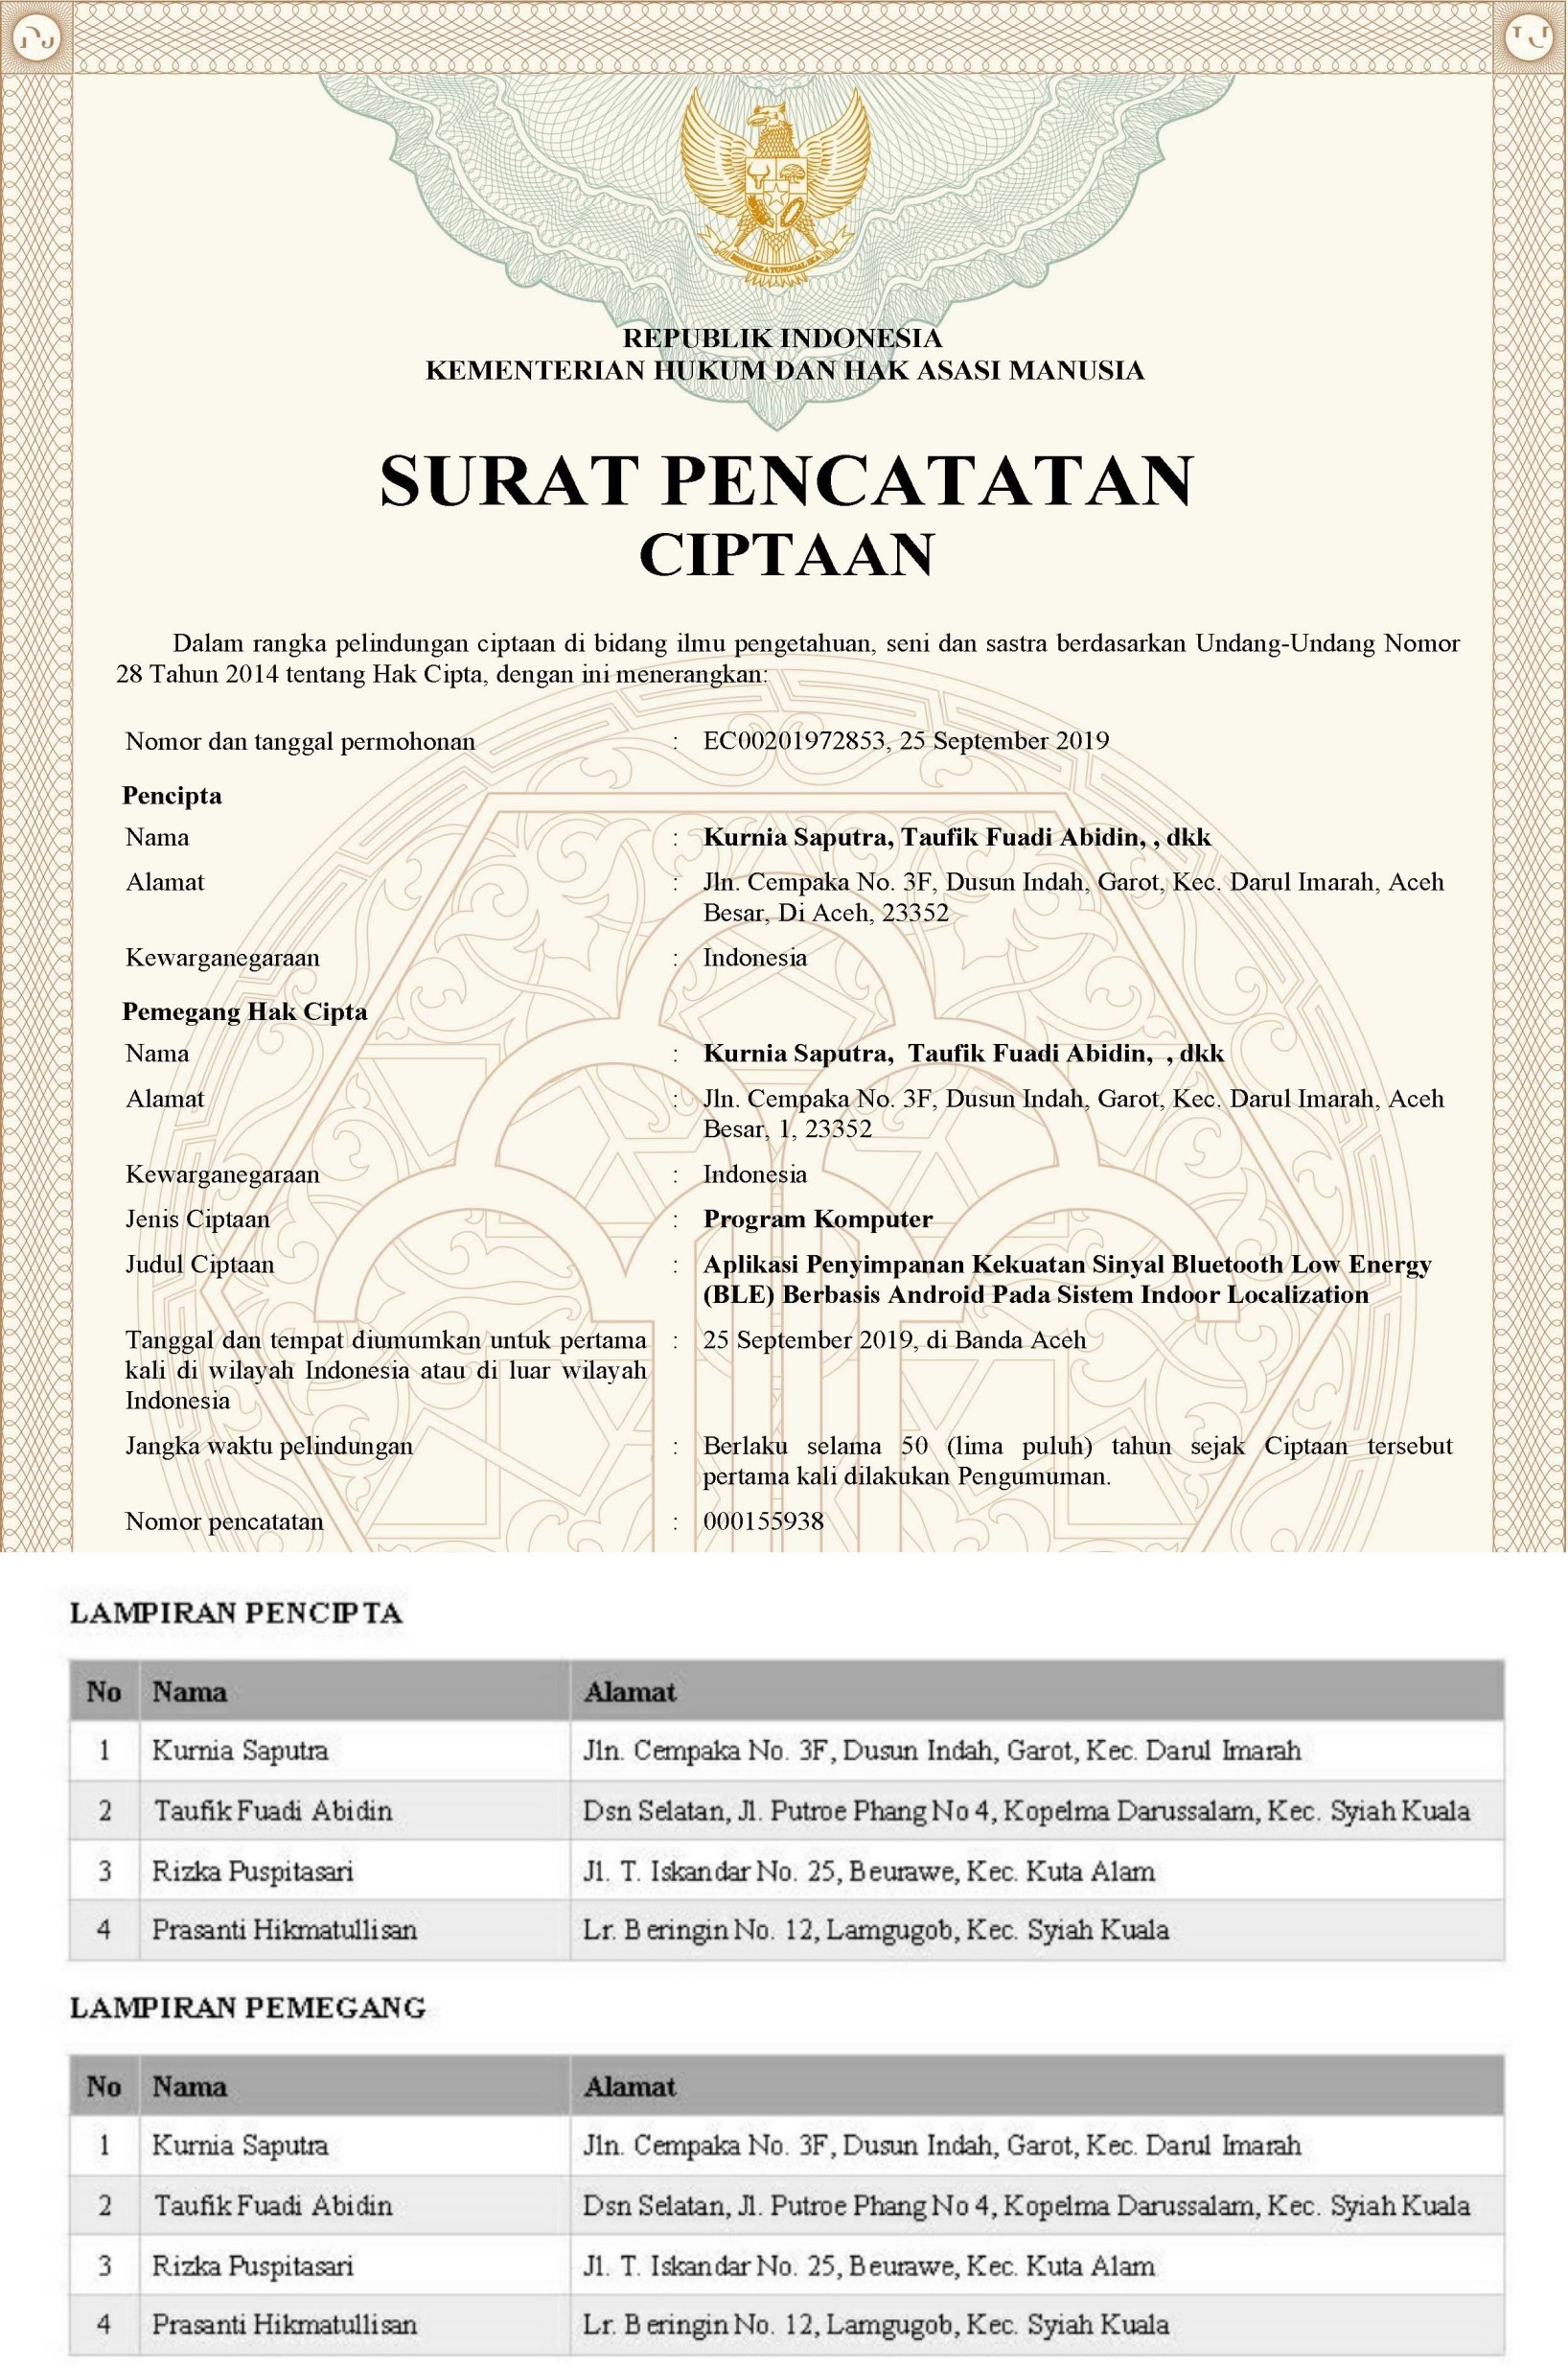
\includegraphics[width = 14cm, height = 21cm]{gambar/lampiran/sertifikat}
% \end{figure}

%------------------------------------------------------%
\addcontentsline{toc}{chapter}{LAMPIRAN 1}
\chapter*{Lampiran 1}
\newappendix{Lampiran 1. Foto Dokumentasi Proses \textit{Mapping}}
\begin{figure}[H]
  \center
  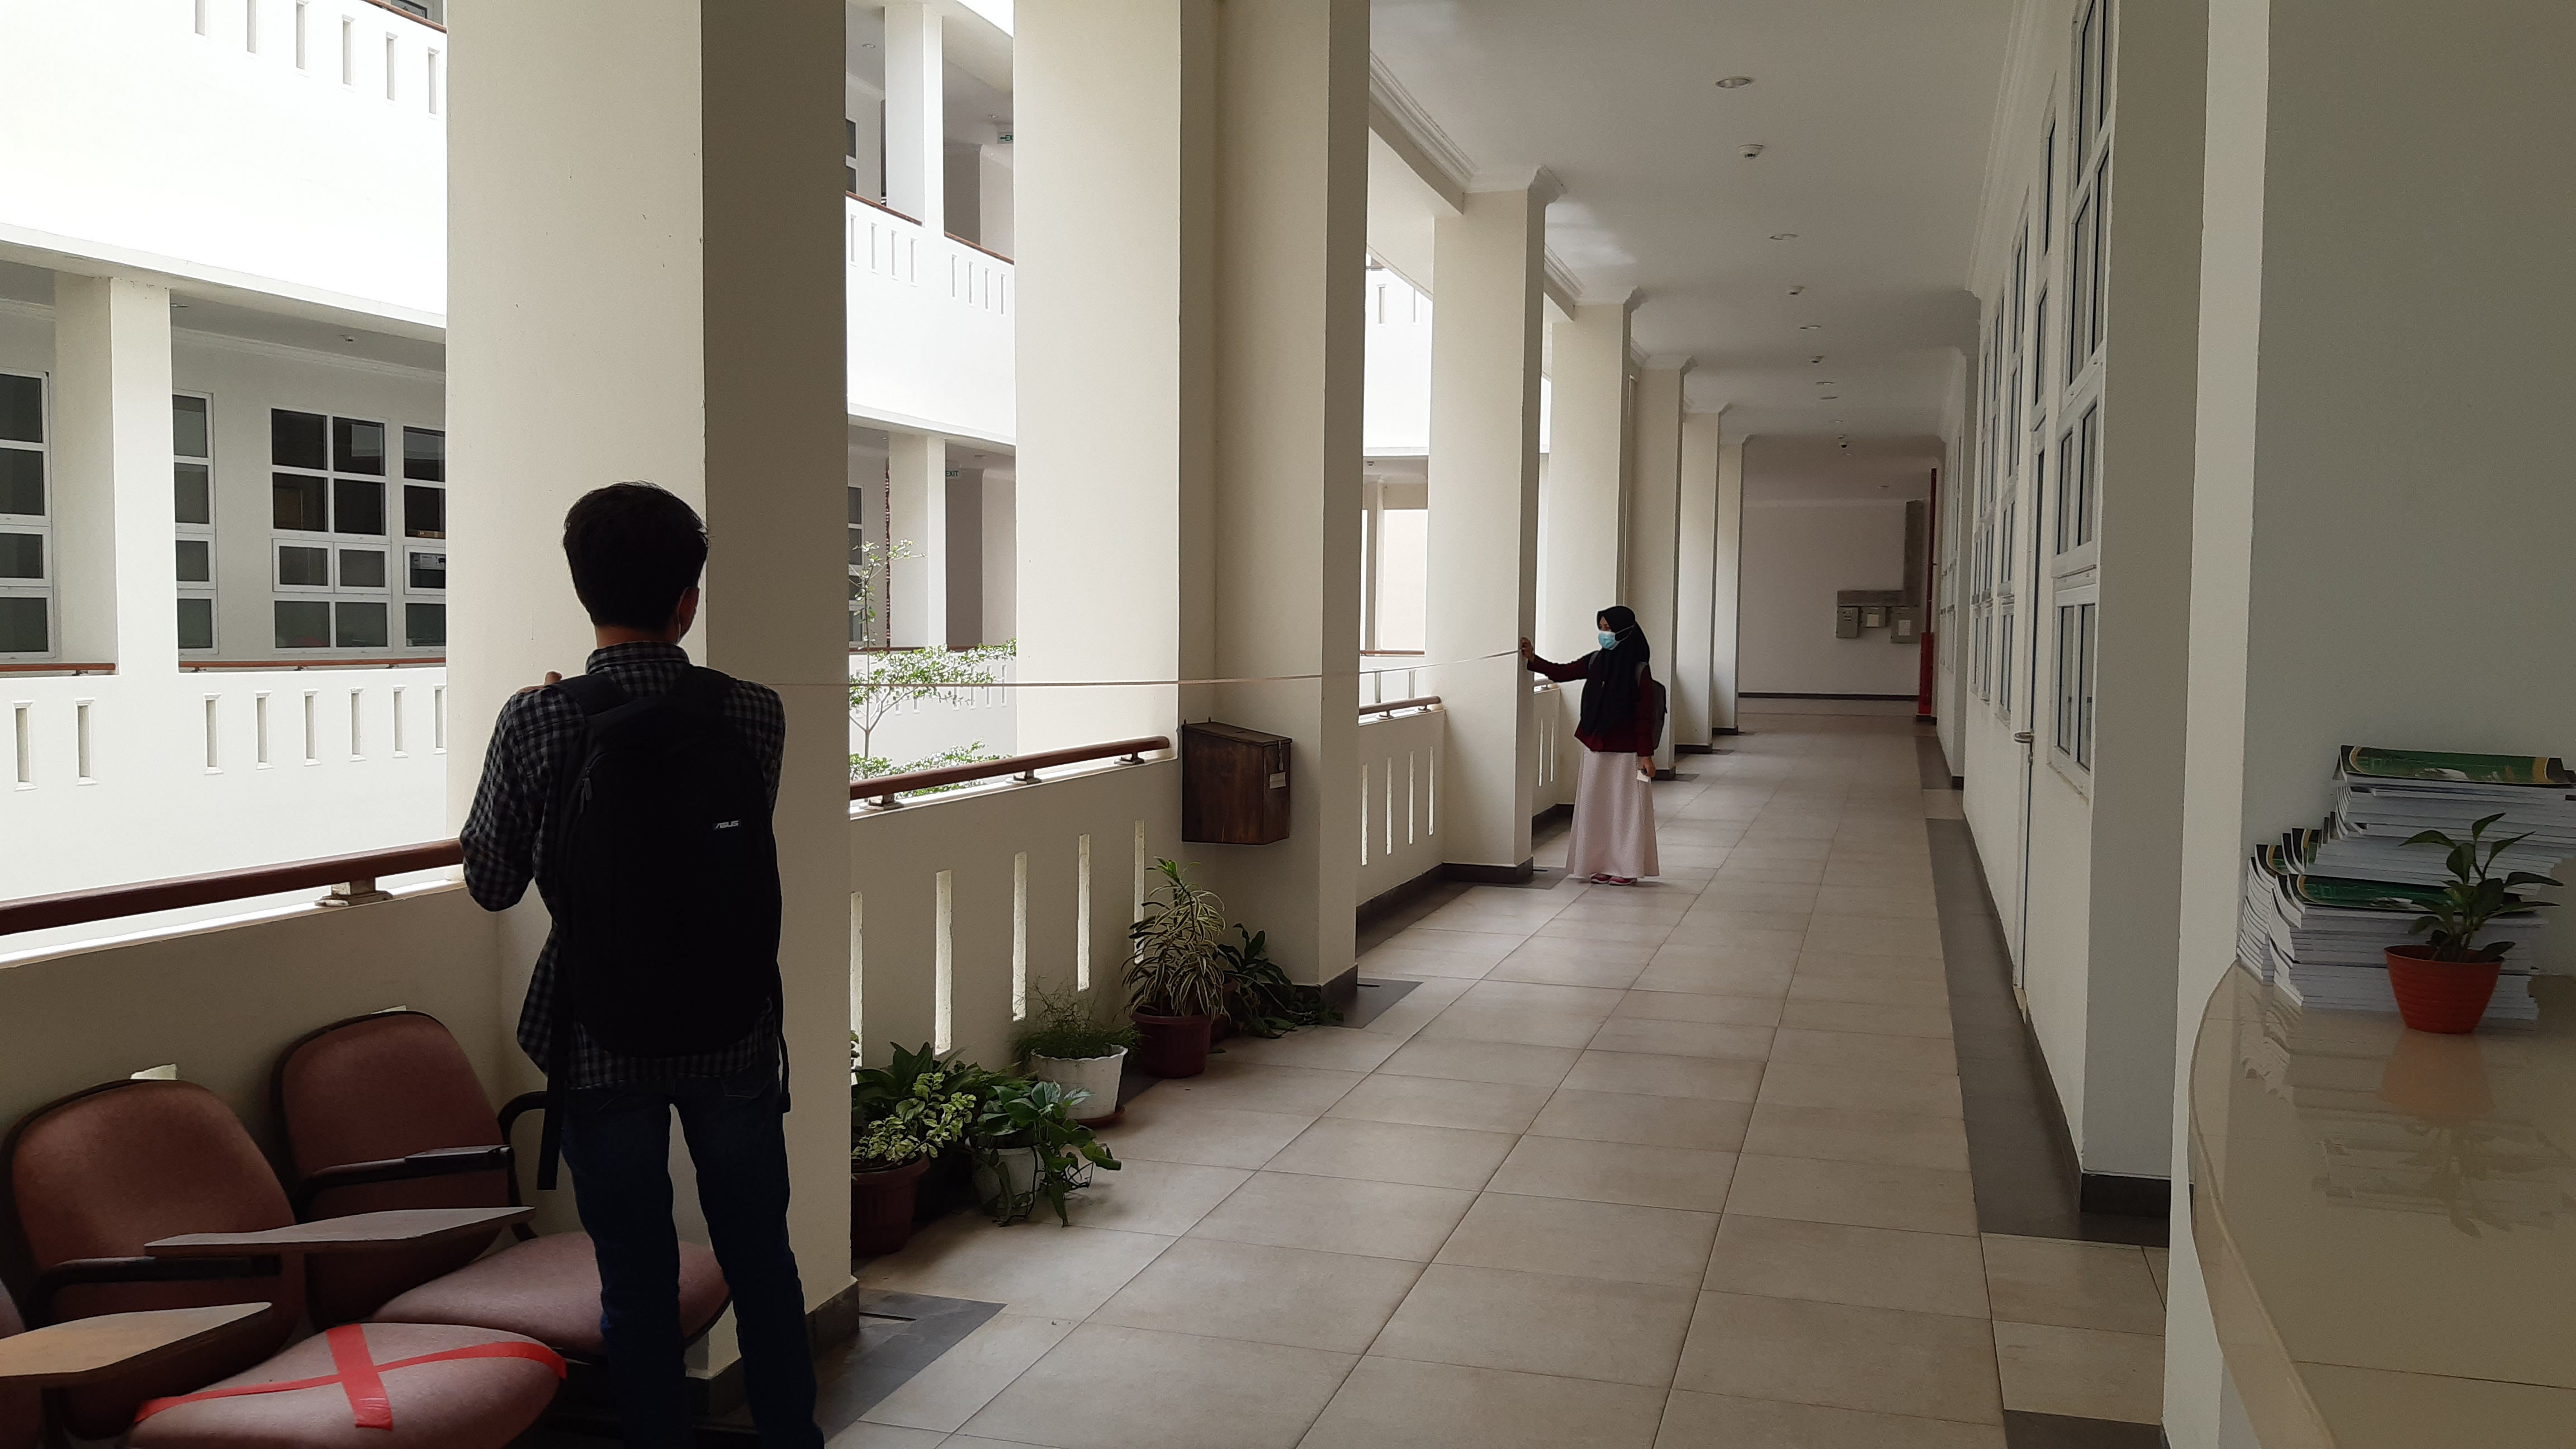
\includegraphics [width = 13.5 cm, height= 6.75 cm]{gambar/lampiran/lamp1a.jpg}
\end{figure}
\begin{figure}[H]
  \center
  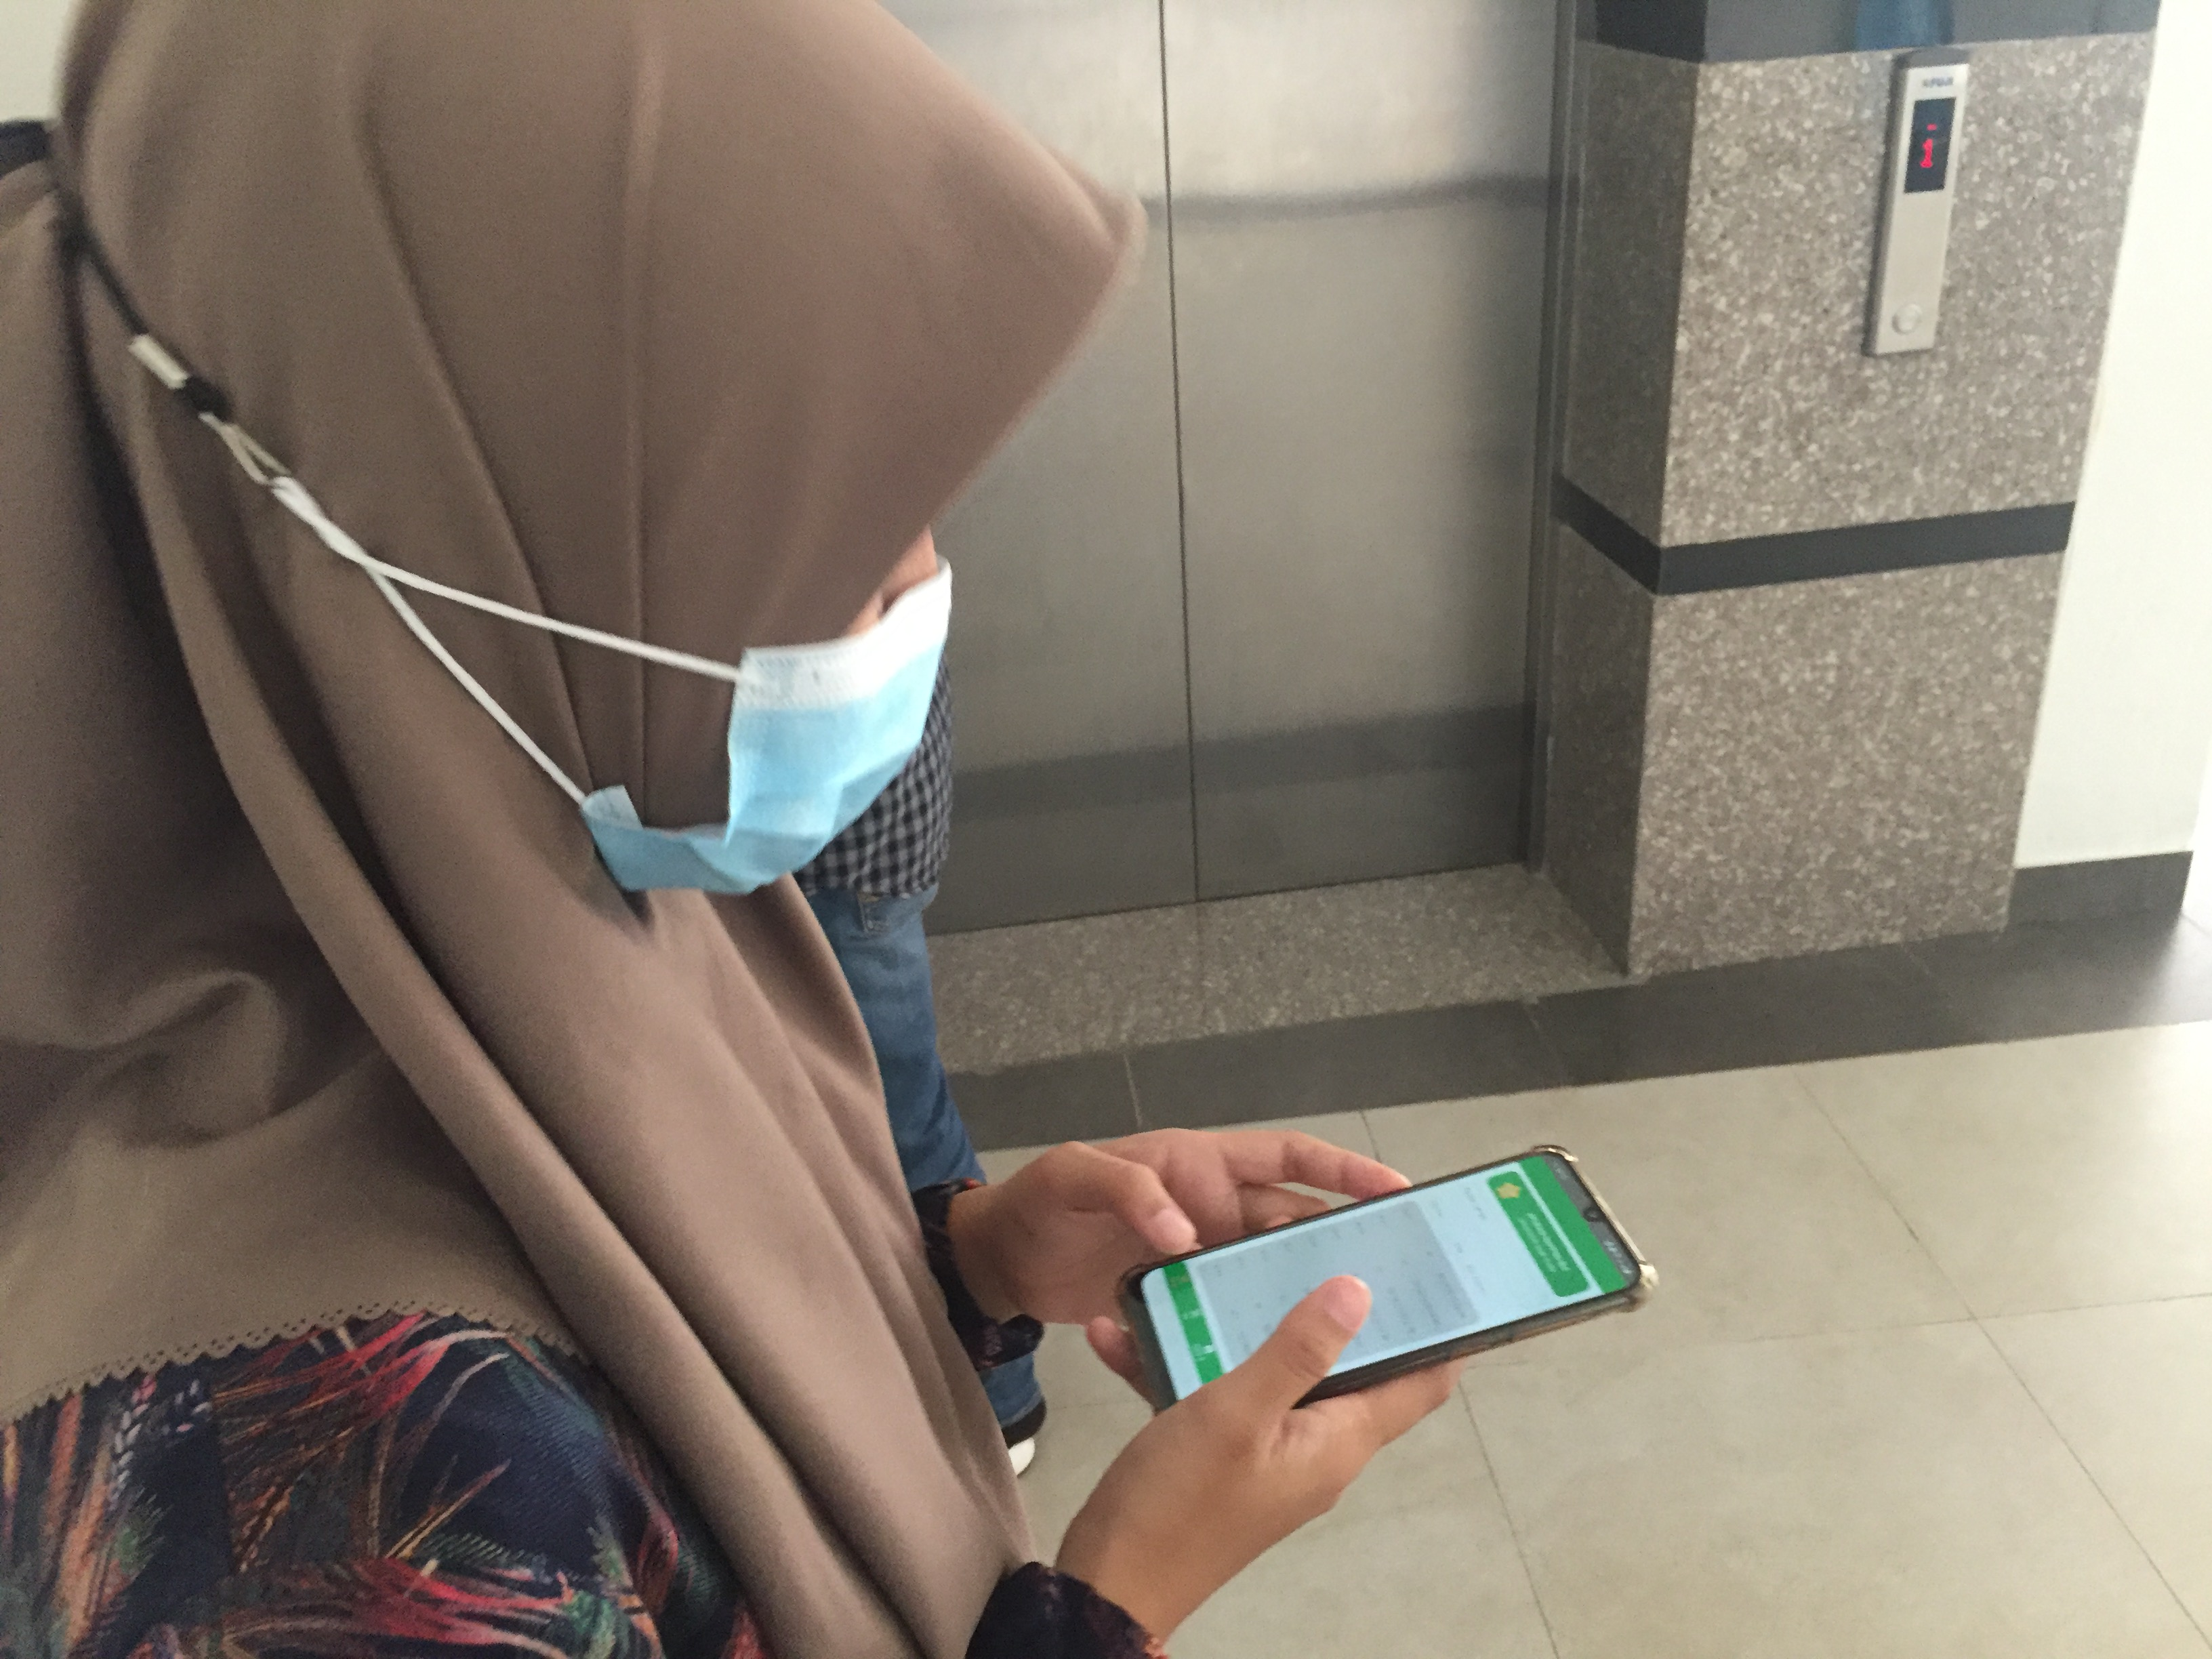
\includegraphics [width = 13.5 cm, height= 6.75 cm]{gambar/lampiran/lamp1d.jpg}
\end{figure}
\begin{figure}[H]
  \center
  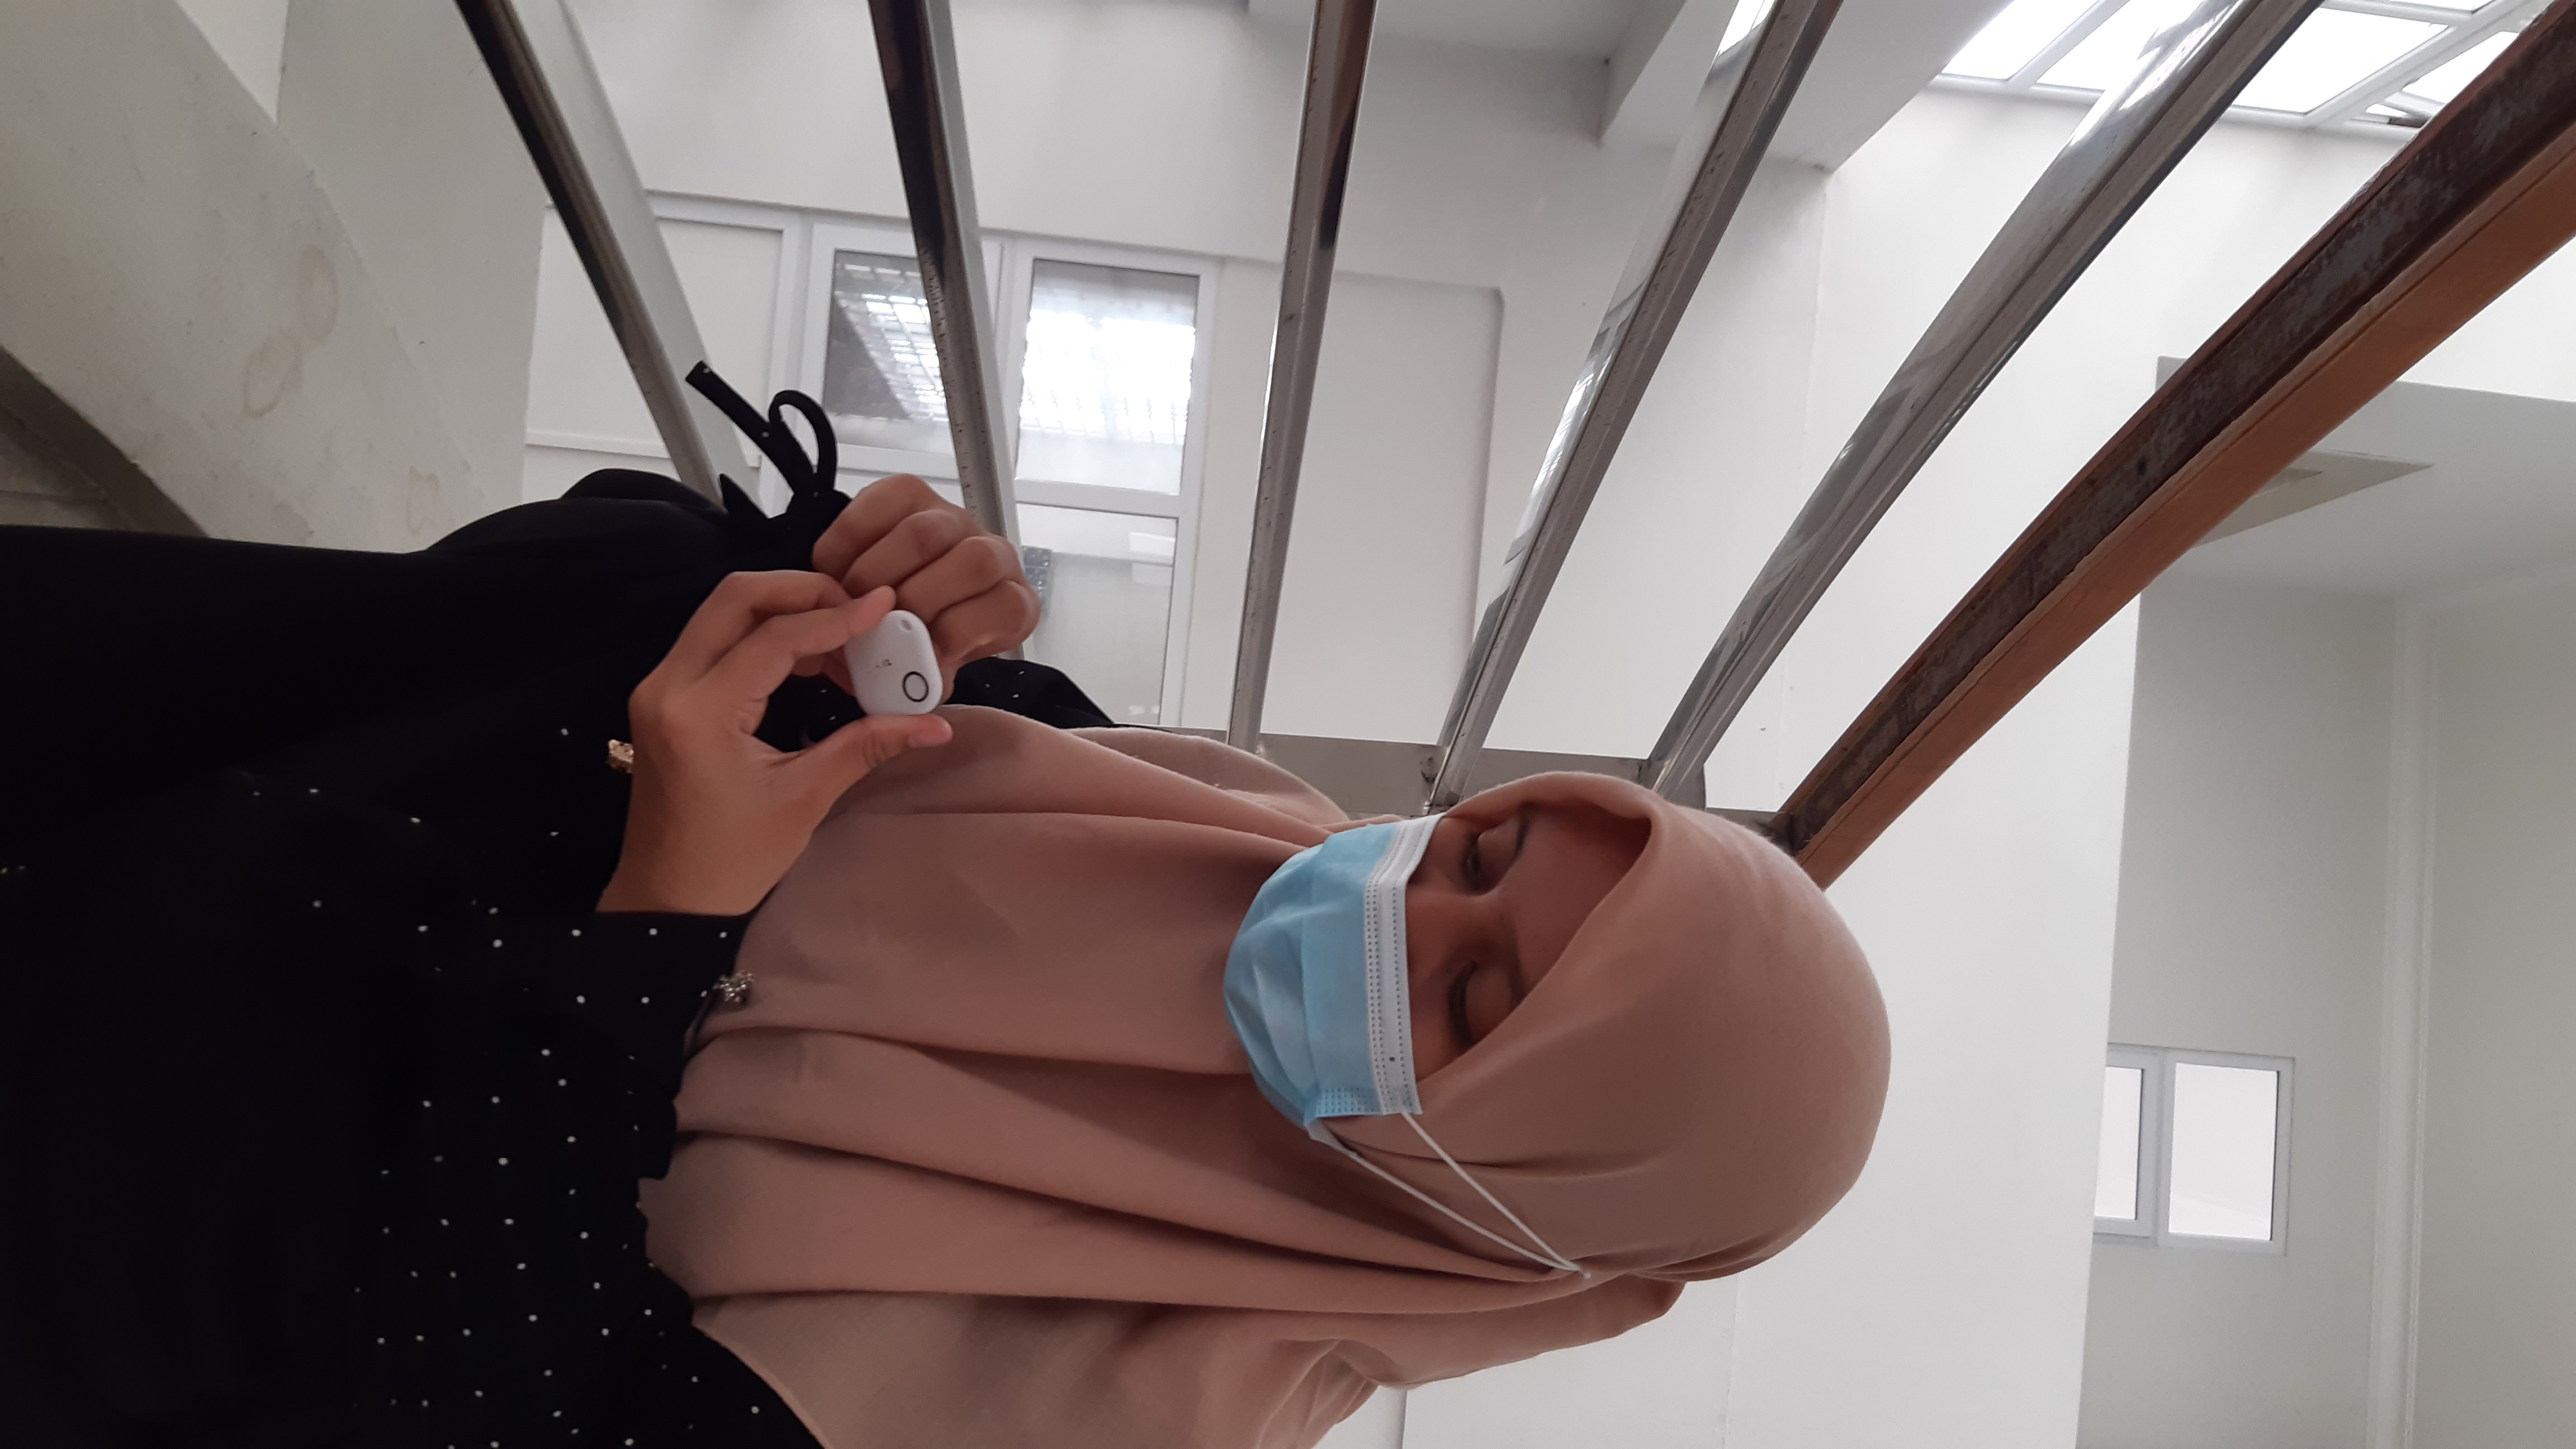
\includegraphics [width = 13.5 cm, height= 6.75 cm]{gambar/lampiran/lamp1b.JPG}
\end{figure}
\label{sus-dosen}



\vspace{2cm}




%-----------------------------------------------------------------------------%
\addcontentsline{toc}{chapter}{LAMPIRAN 2}
\chapter*{Lampiran 2}
\newappendix{Lampiran 2. Foto Dokumentasi Proses Pengujian  \textit{Usability} dan Fungsionalitas}

\begin{figure}[H]
  \center
  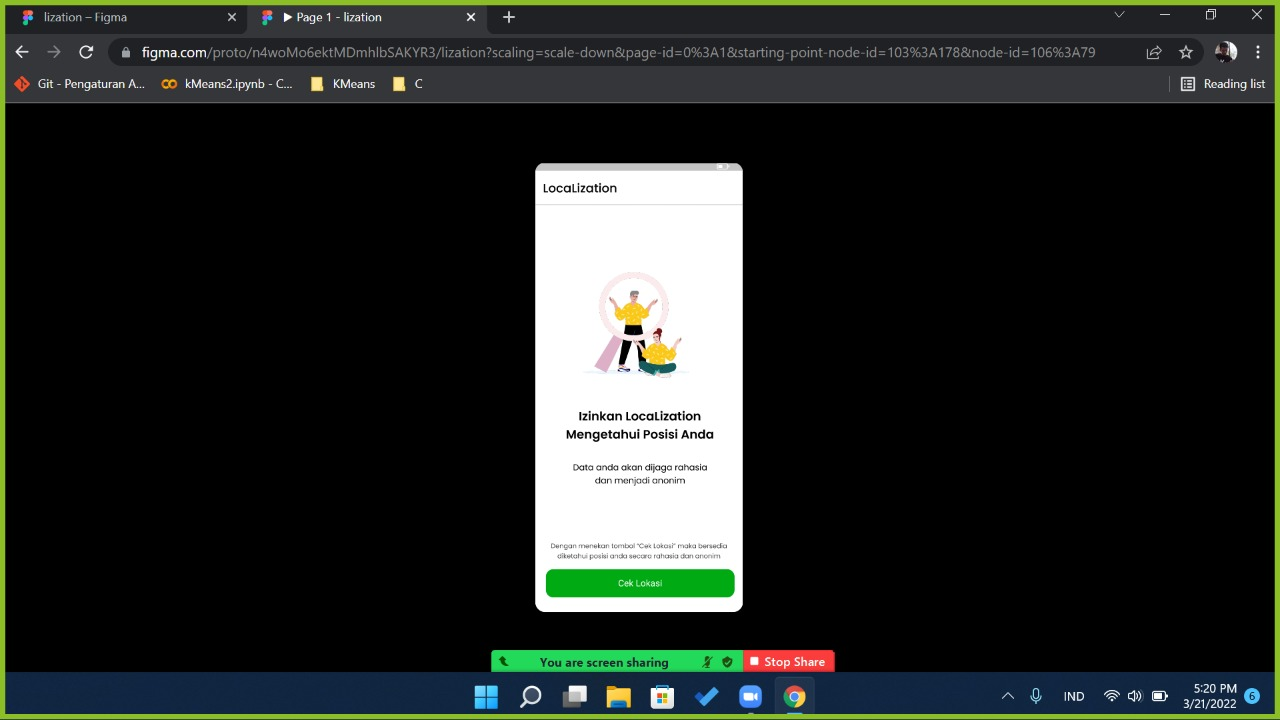
\includegraphics [width = 13.5 cm, height= 6.75 cm]{gambar/lampiran/umux1.jpeg}
\end{figure}
\begin{figure}[H]
  \center
  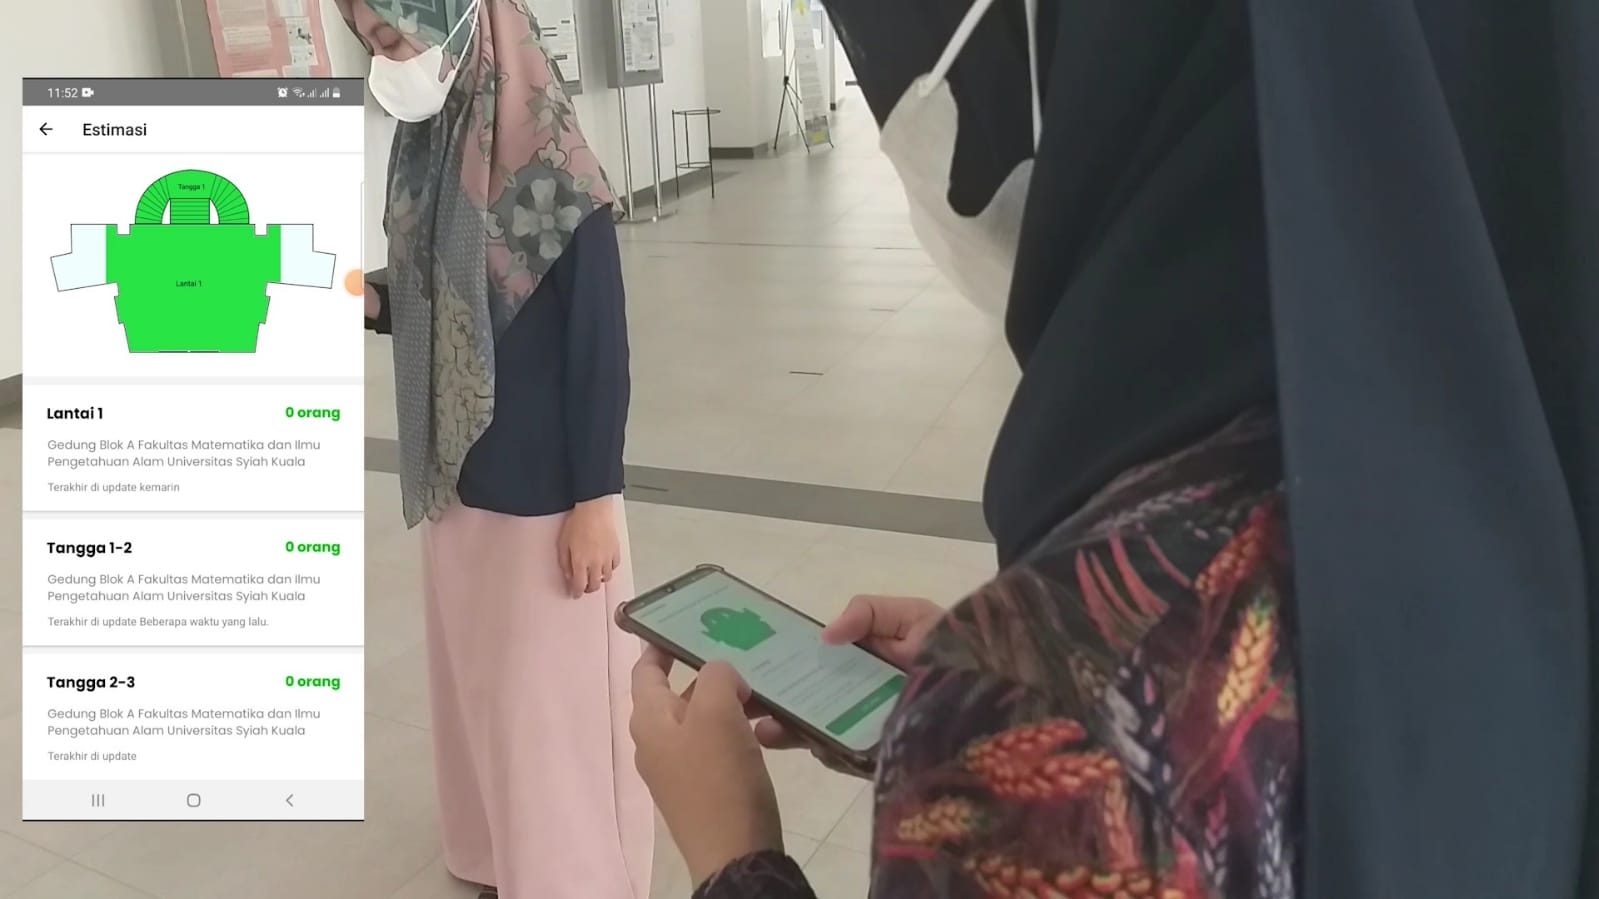
\includegraphics [width = 13.5 cm, height= 6.75 cm]{gambar/lampiran/umux5.jpeg}
\end{figure}
\begin{figure}[H]
  \center
  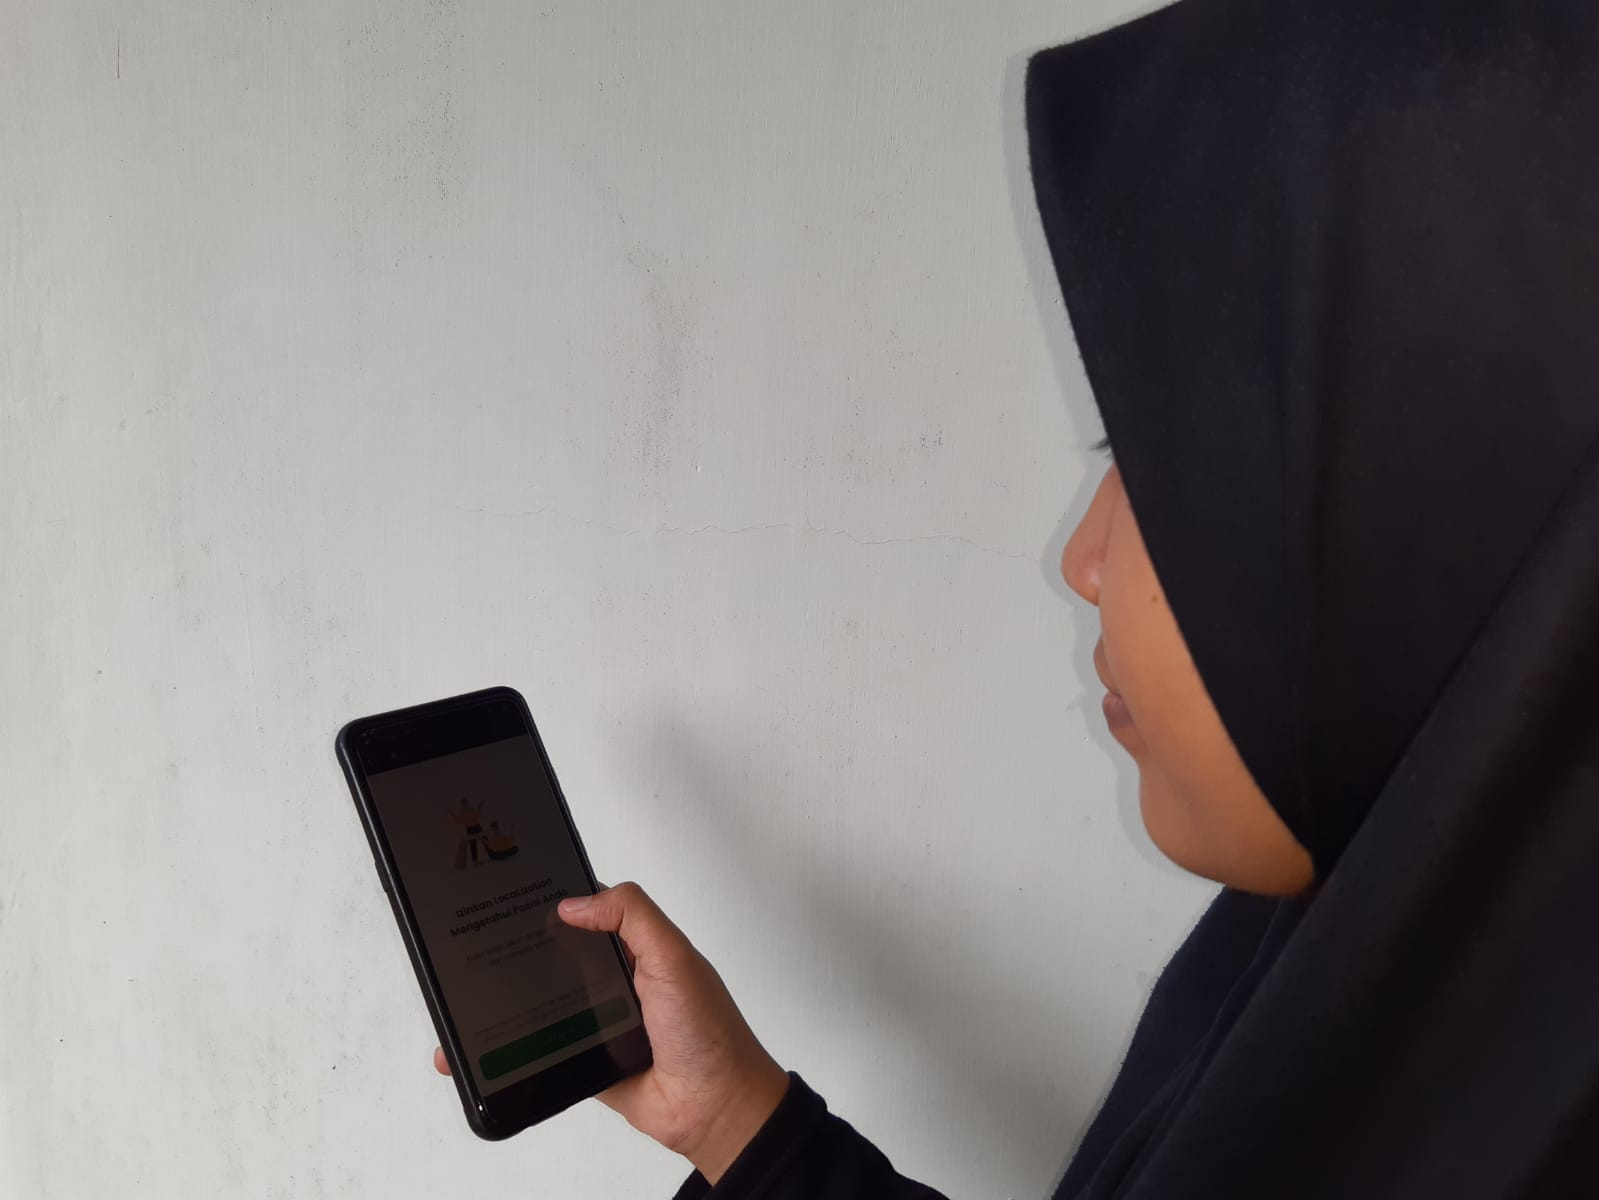
\includegraphics [width = 13.5 cm, height= 6.75 cm]{gambar/lampiran/umux3.jpeg}
\end{figure}
\label{sus-dosen}
\begin{figure}[H]
  \center
  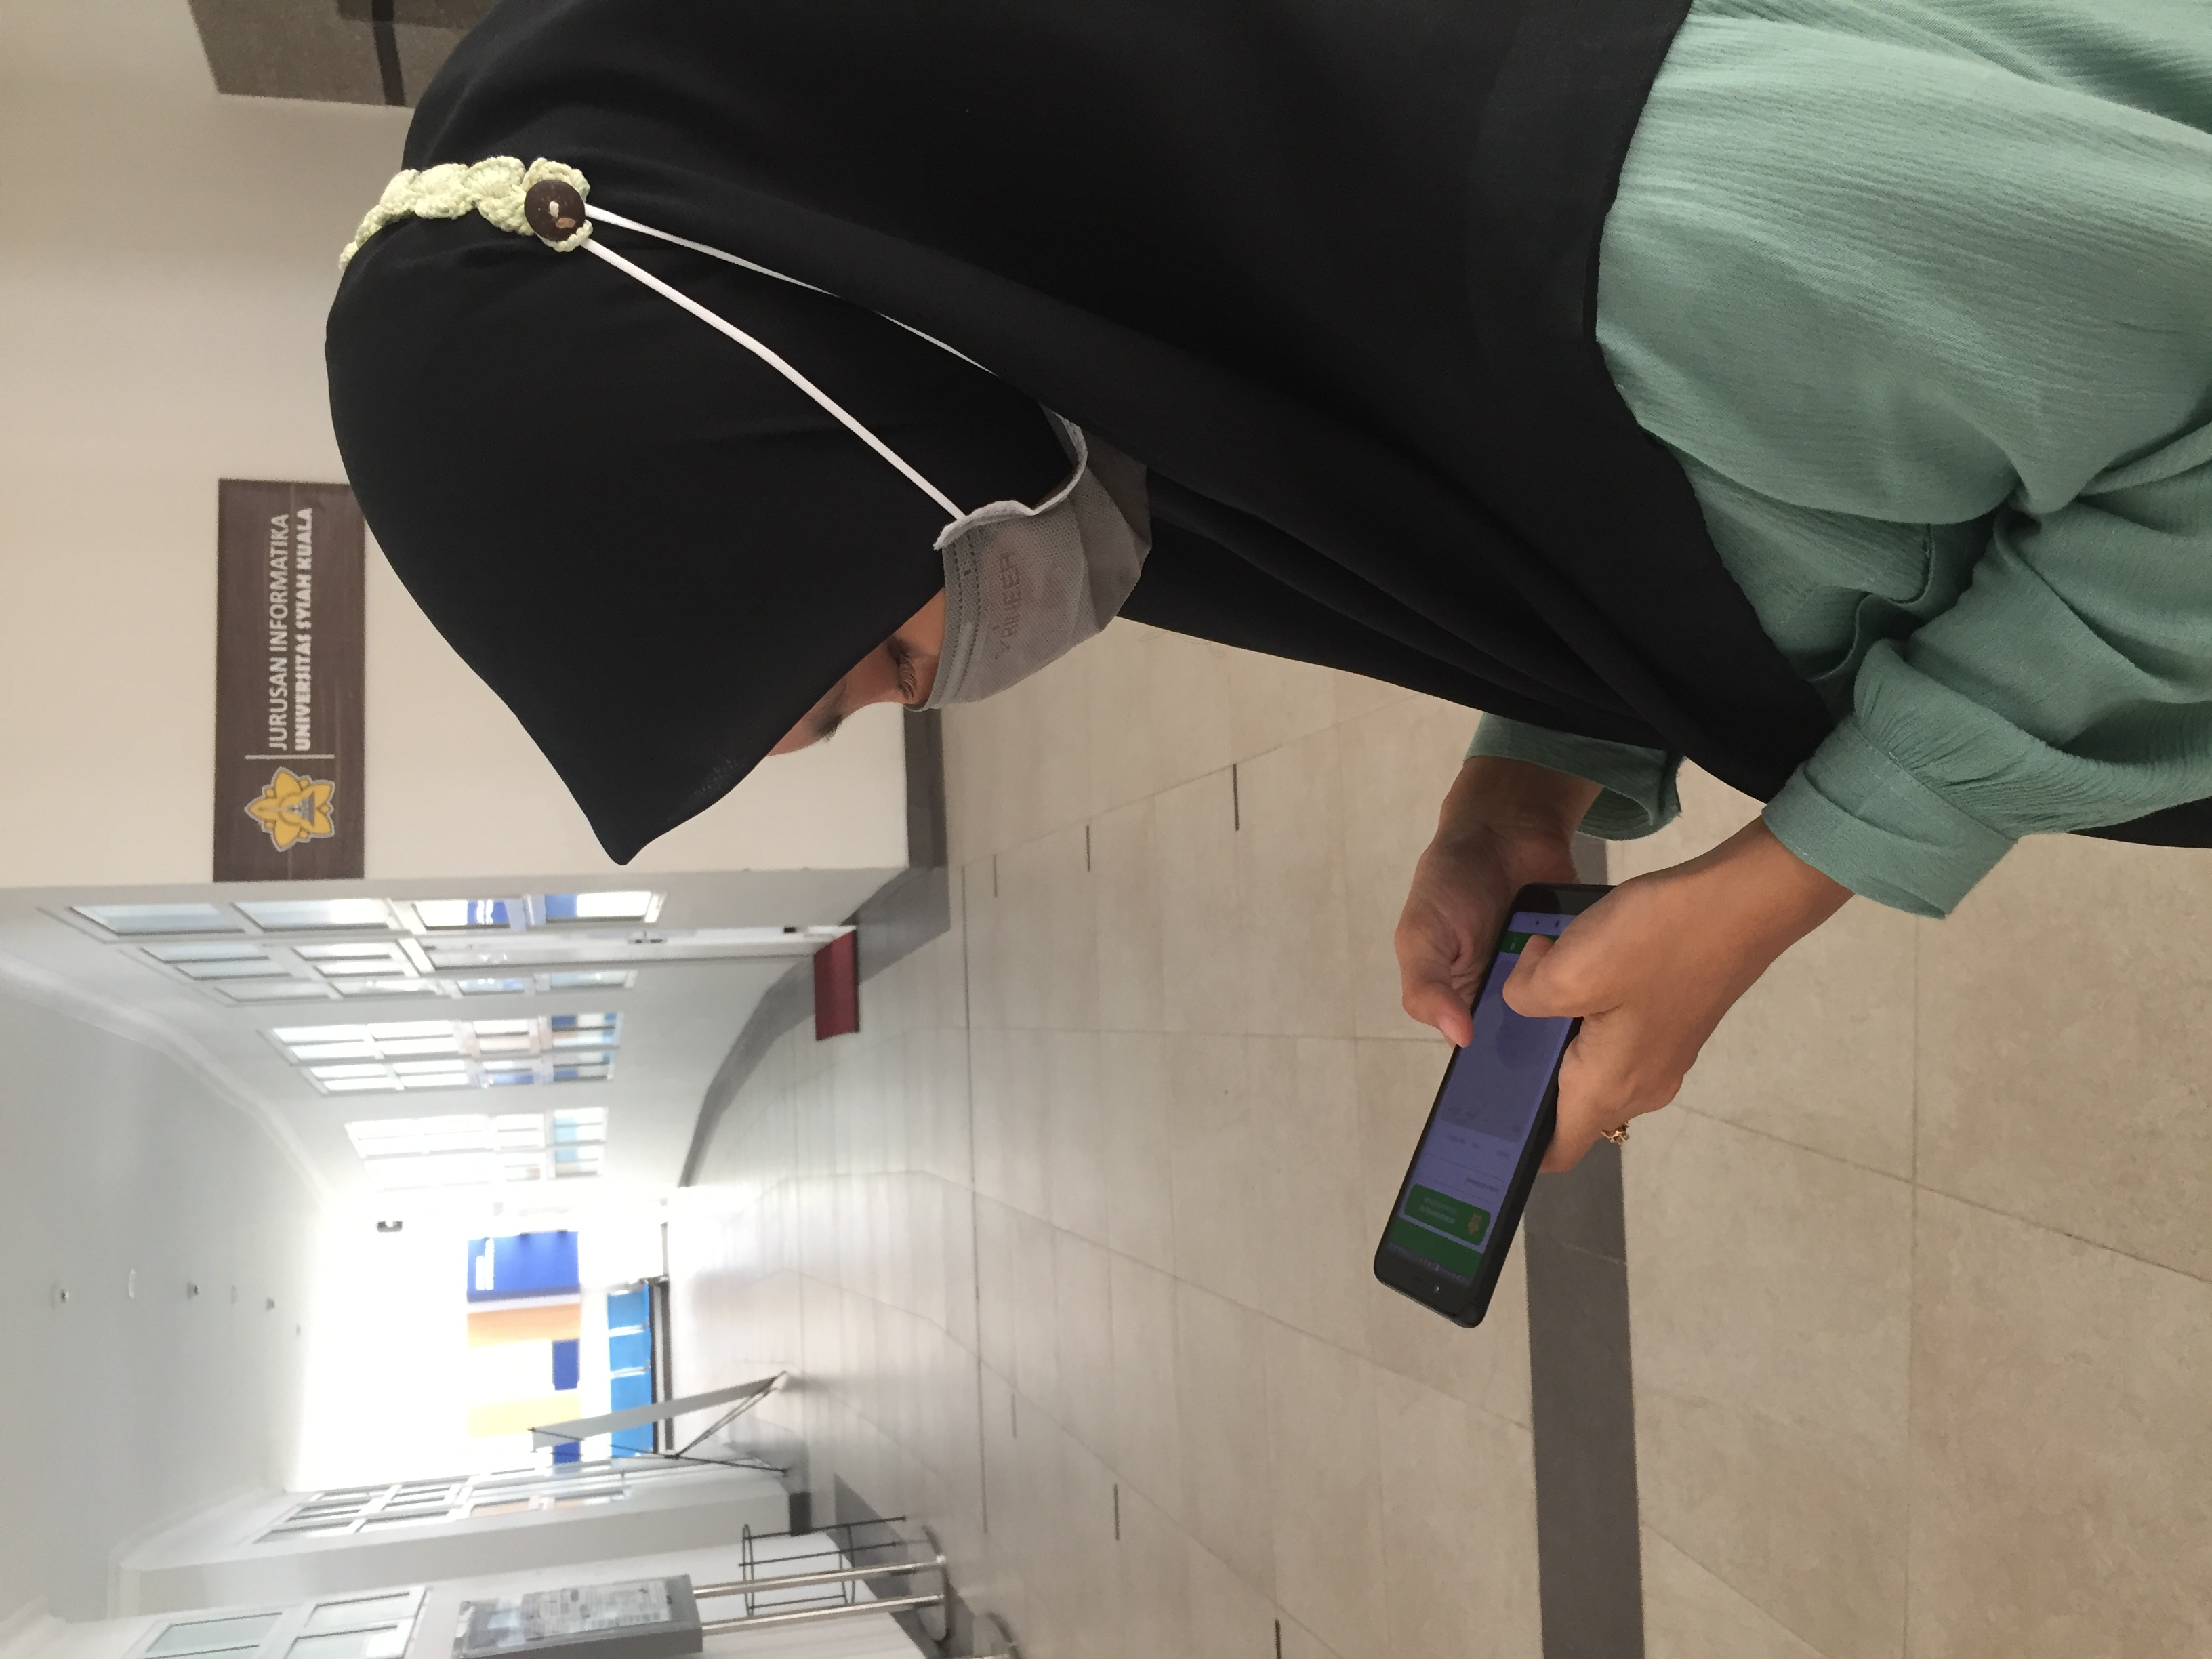
\includegraphics [width = 13.5 cm, height= 6.75 cm]{gambar/lampiran/umux4.JPG}
\end{figure}
\begin{figure}[H]
  \center
  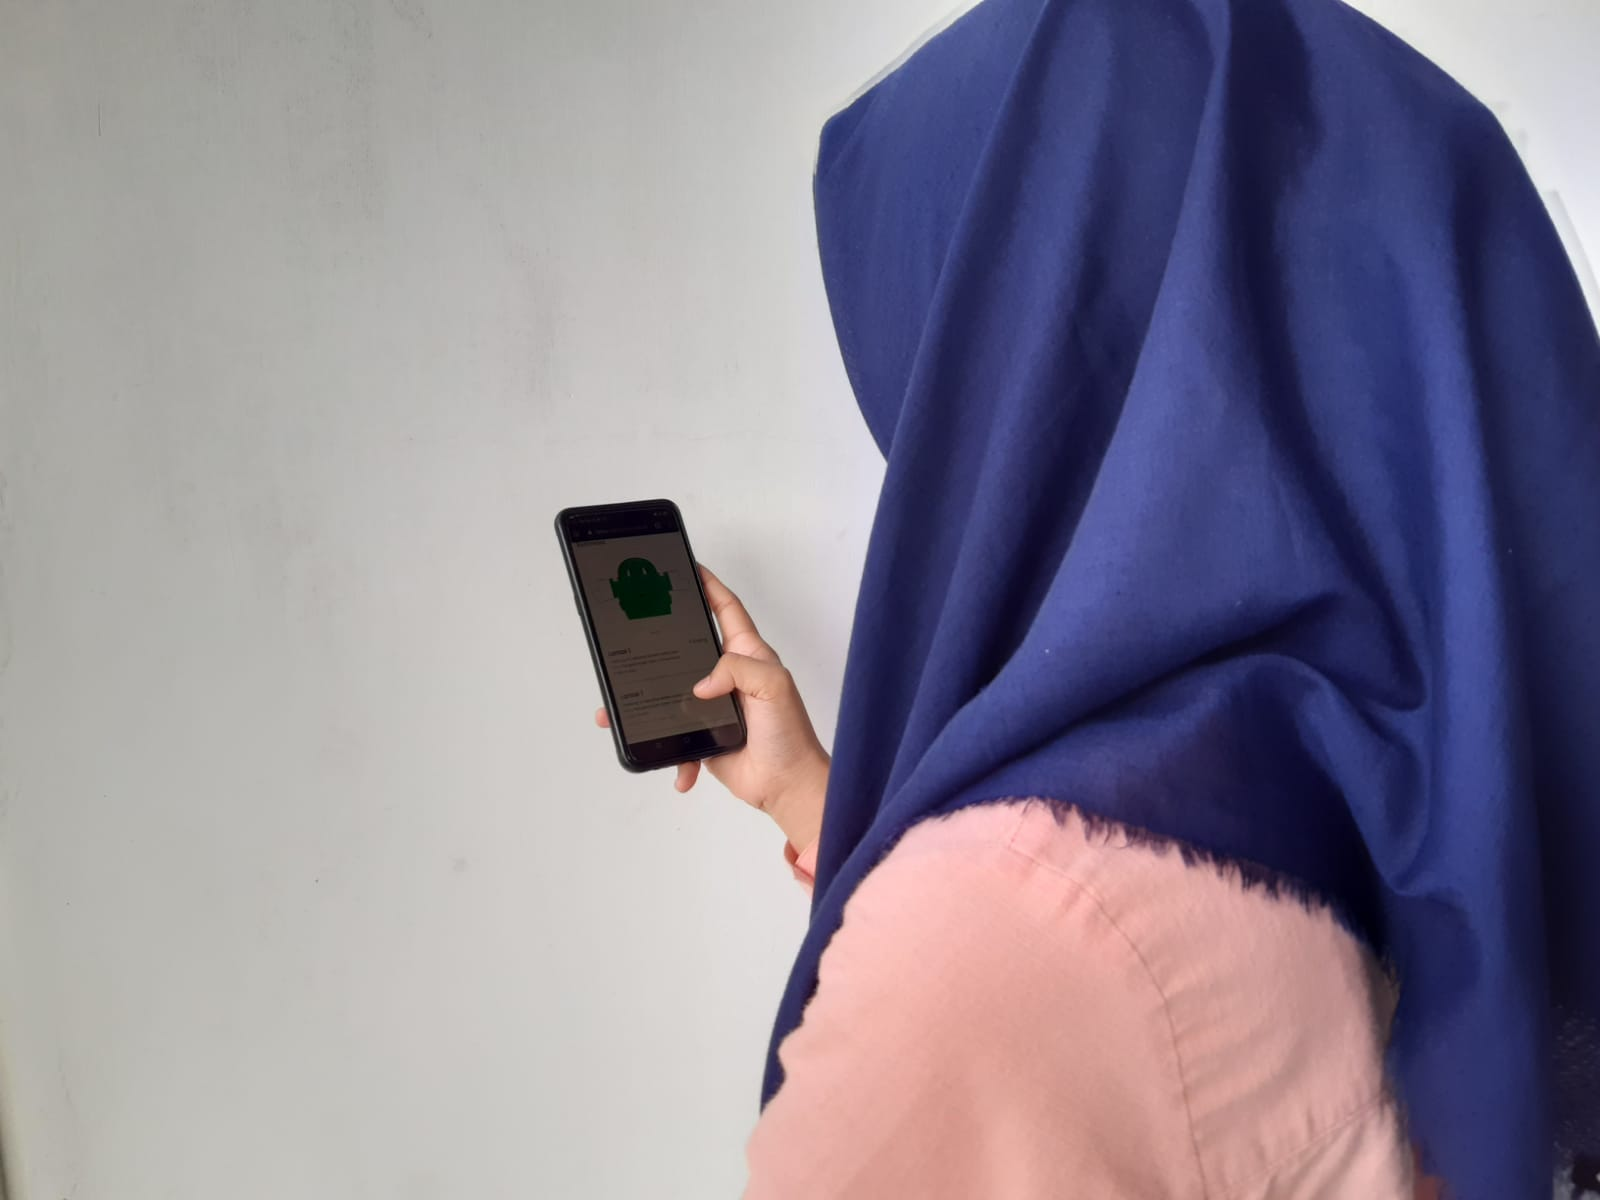
\includegraphics [width = 13.5 cm, height= 6.75 cm]{gambar/lampiran/umux2.jpeg}
\end{figure}
\begin{figure}[H]
  \center
  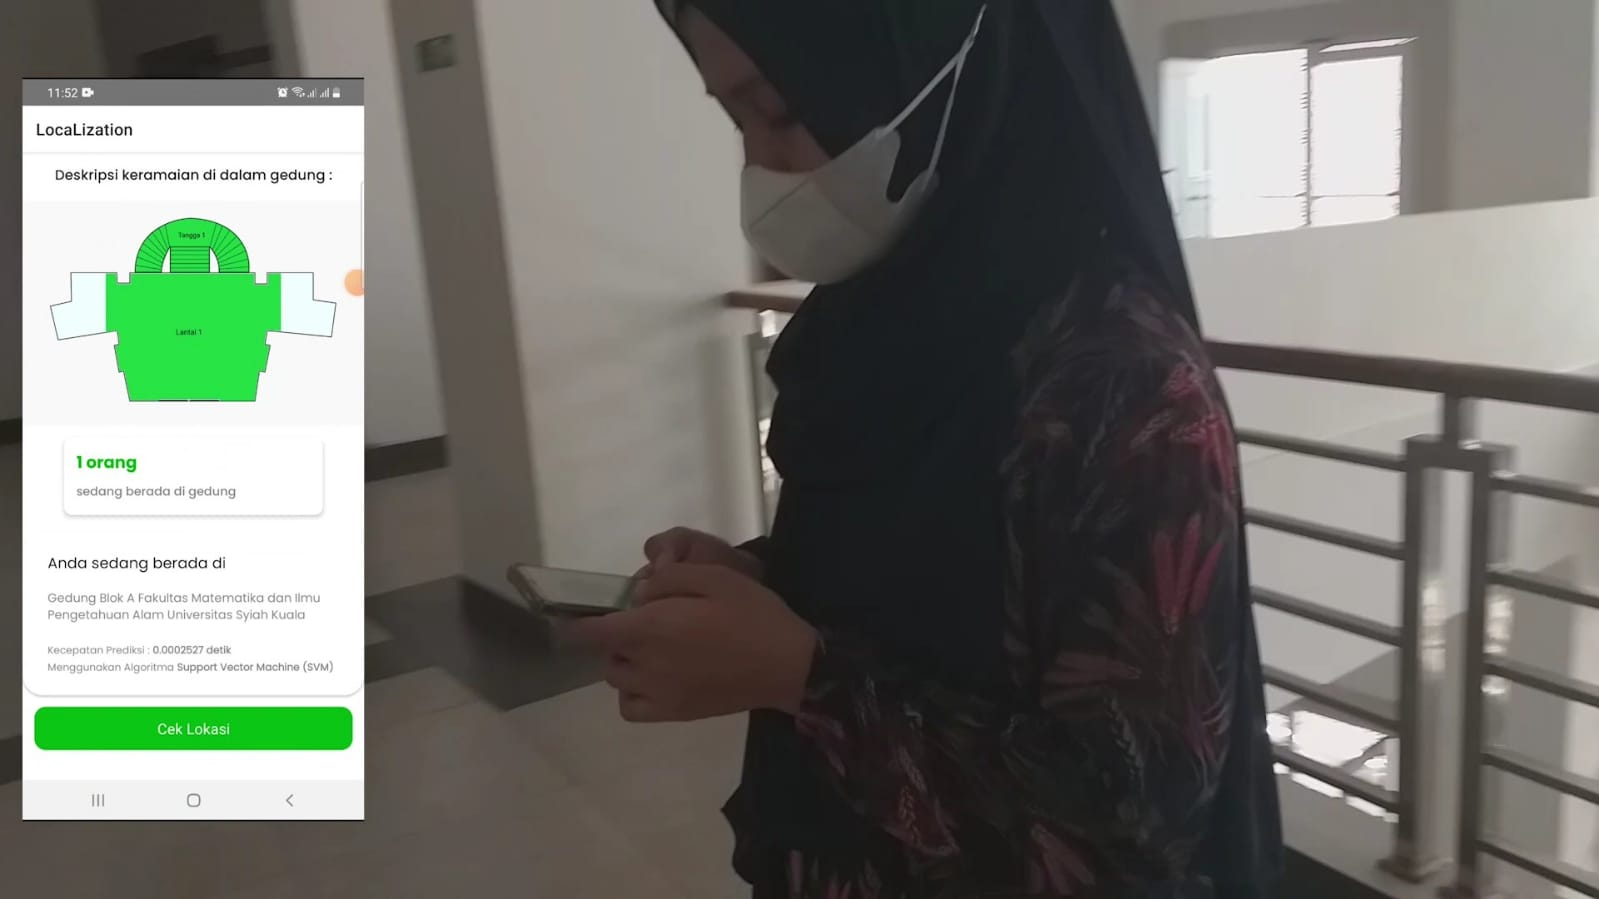
\includegraphics [width = 13.5 cm, height= 6.75 cm]{gambar/lampiran/umux6.jpeg}
\end{figure}
% \label{sus-mahasiswa}


%-----------------------------------------------------------------------------%

\addcontentsline{toc}{chapter}{LAMPIRAN 3}
\chapter*{Lampiran 3}
\newappendix{Lampiran 3. Foto Dokumentasi Scrum}
% \begin{figure}[htp]
\centering
\vspace{0.4cm}

\begin{figure}[H]
  \center
  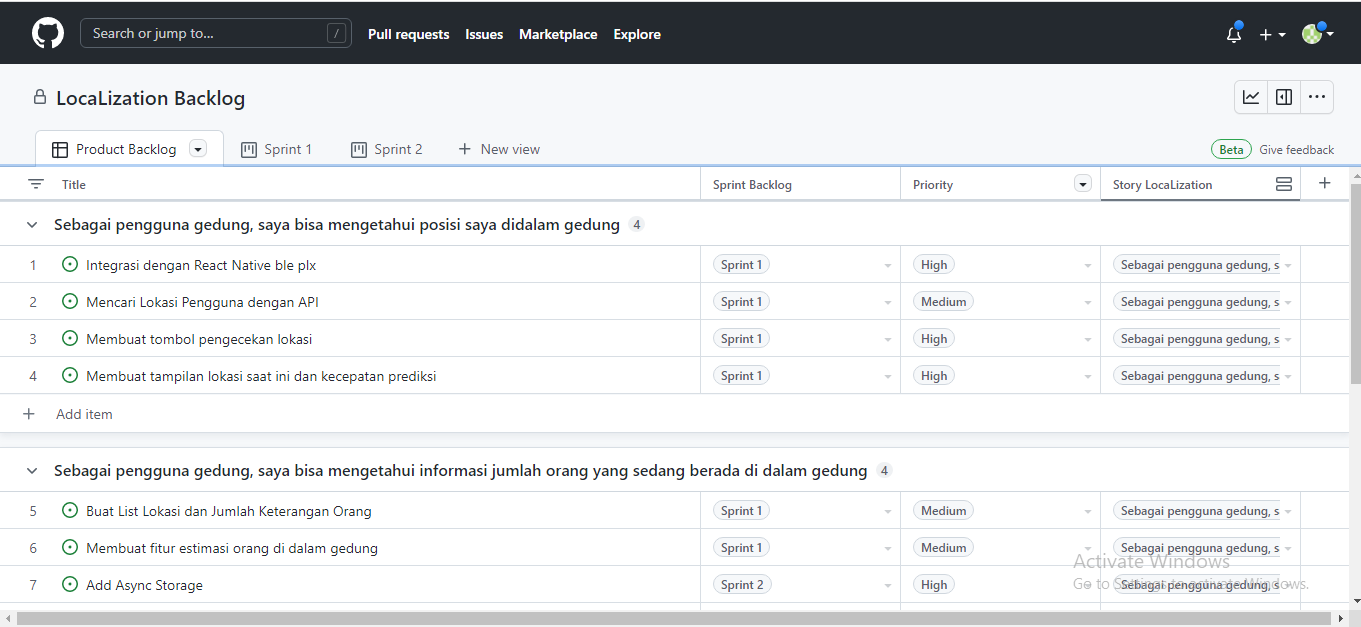
\includegraphics [width = 13.5 cm, height= 6.75 cm]{gambar/lampiran/scrum1.PNG}
\end{figure}
\begin{figure}[H]
  \center
  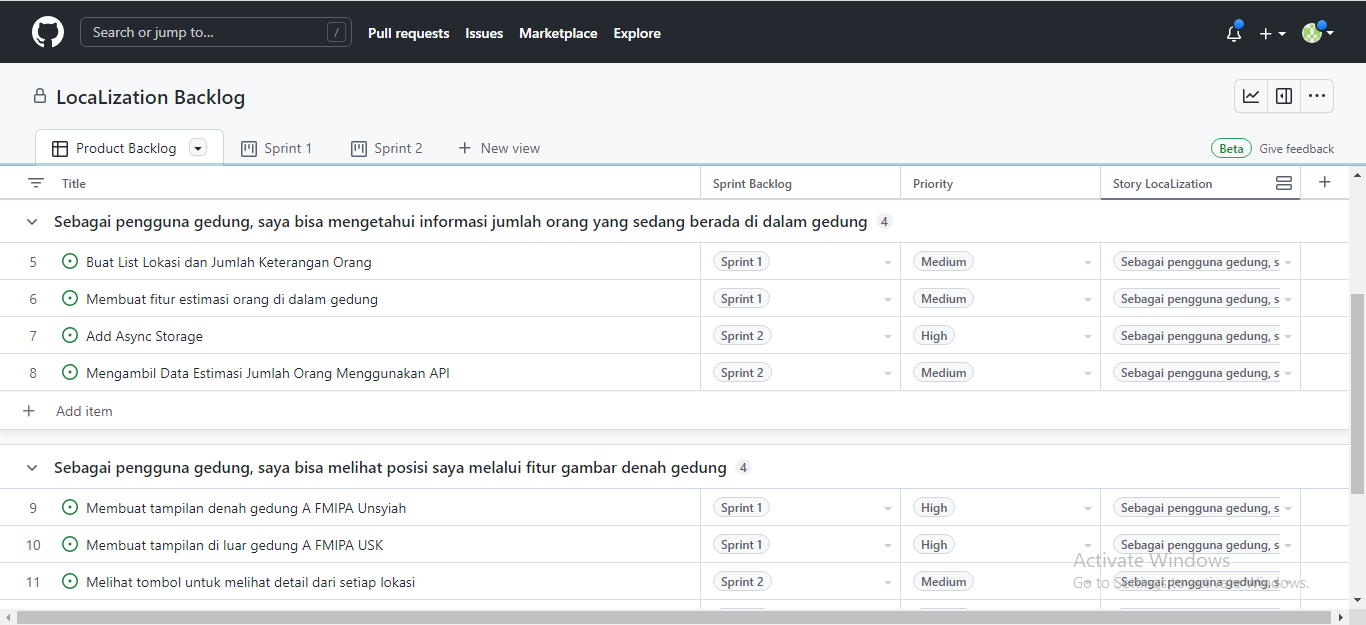
\includegraphics [width = 13.5 cm, height= 6.75 cm]{gambar/lampiran/scrum2.PNG}
\end{figure}
\begin{figure}[H]
  \center
  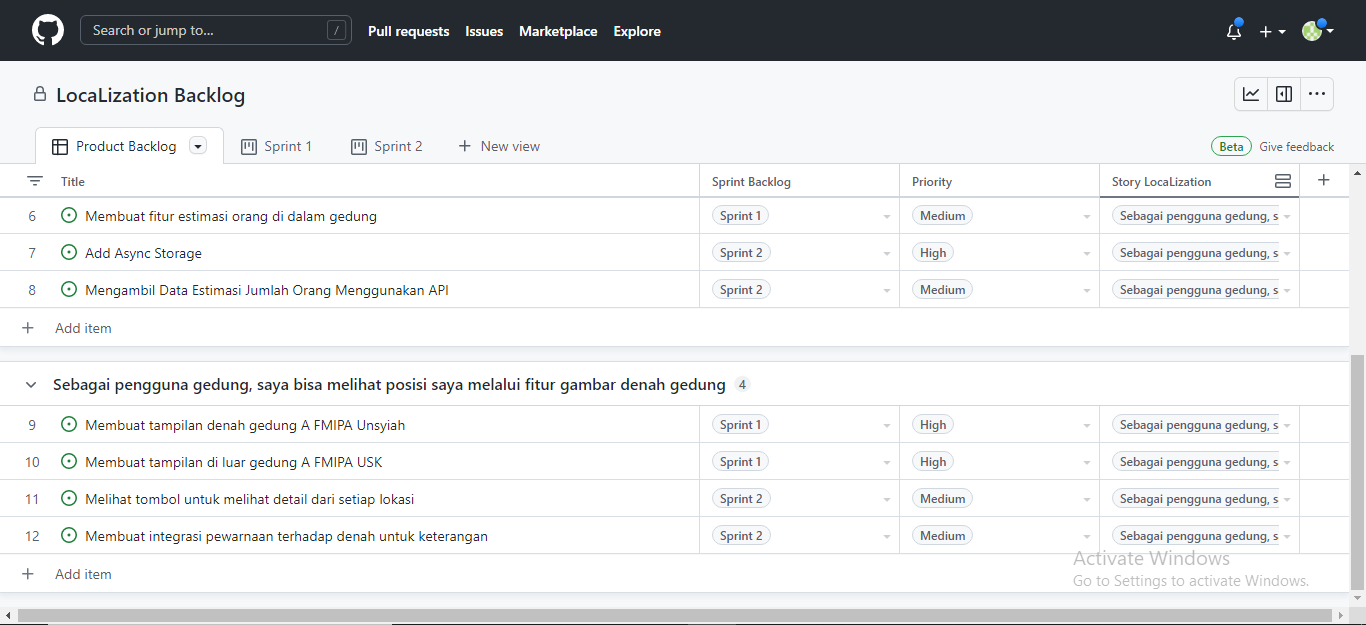
\includegraphics [width = 13.5 cm, height= 6.75 cm]{gambar/lampiran/scrum3.PNG}
\end{figure}
\begin{figure}[H]
  \center
  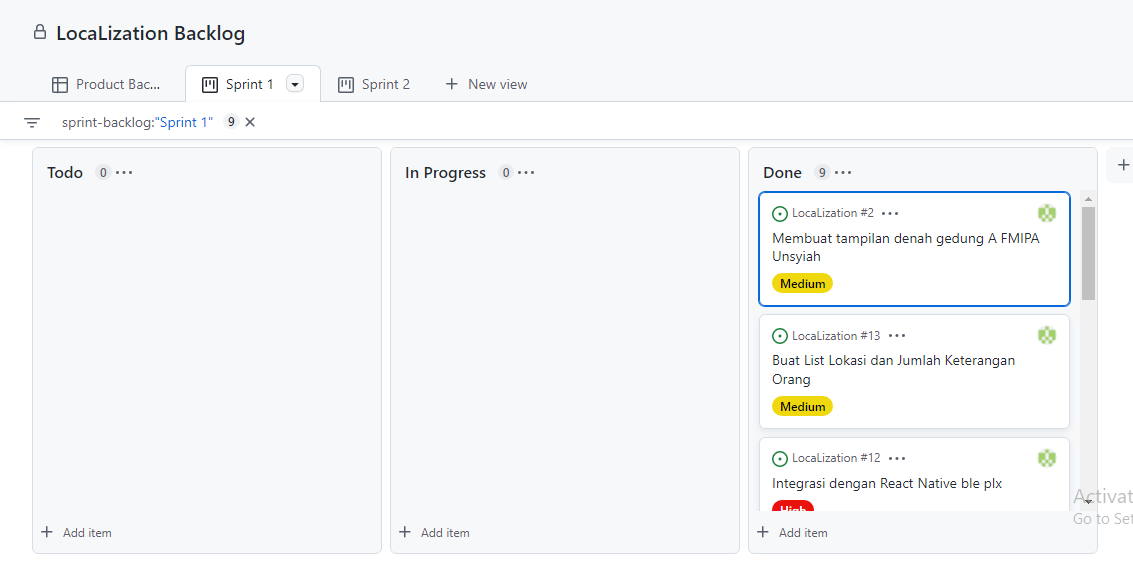
\includegraphics [width = 13.5 cm, height= 6.75 cm]{gambar/lampiran/sprint1.PNG}
\end{figure}
\begin{figure}[H]
  \center
  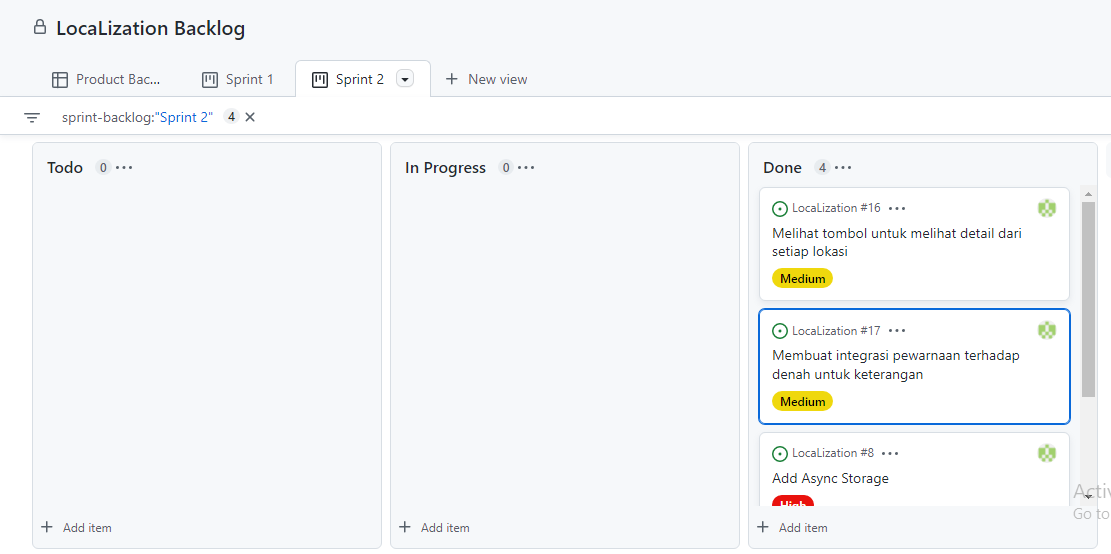
\includegraphics [width = 13.5 cm, height= 6.75 cm]{gambar/lampiran/sprint2.PNG}
\end{figure}

% \end{figure}
%-----------------------------------------------------------------------------%

\addcontentsline{toc}{chapter}{LAMPIRAN 4}
\chapter*{Lampiran 4}
\newappendix{Lampiran 4. Foto Bukti Fisik ALat Pemancar Sinyal BLE atau Beacon }
% \begin{figure}[htp]
\centering
\vspace{0.4cm}

\begin{figure}[H]
  \center
  \includegraphics [width = 13.5 cm, height= 7 cm]{gambar/lampiran/ble1.jpg}
\end{figure}
\begin{figure}[H]
  \center
  \includegraphics [width = 13.5 cm, height= 7 cm]{gambar/lampiran/ble2.jpg}
\end{figure}

% Lampiran 4 Laporan Usability

% 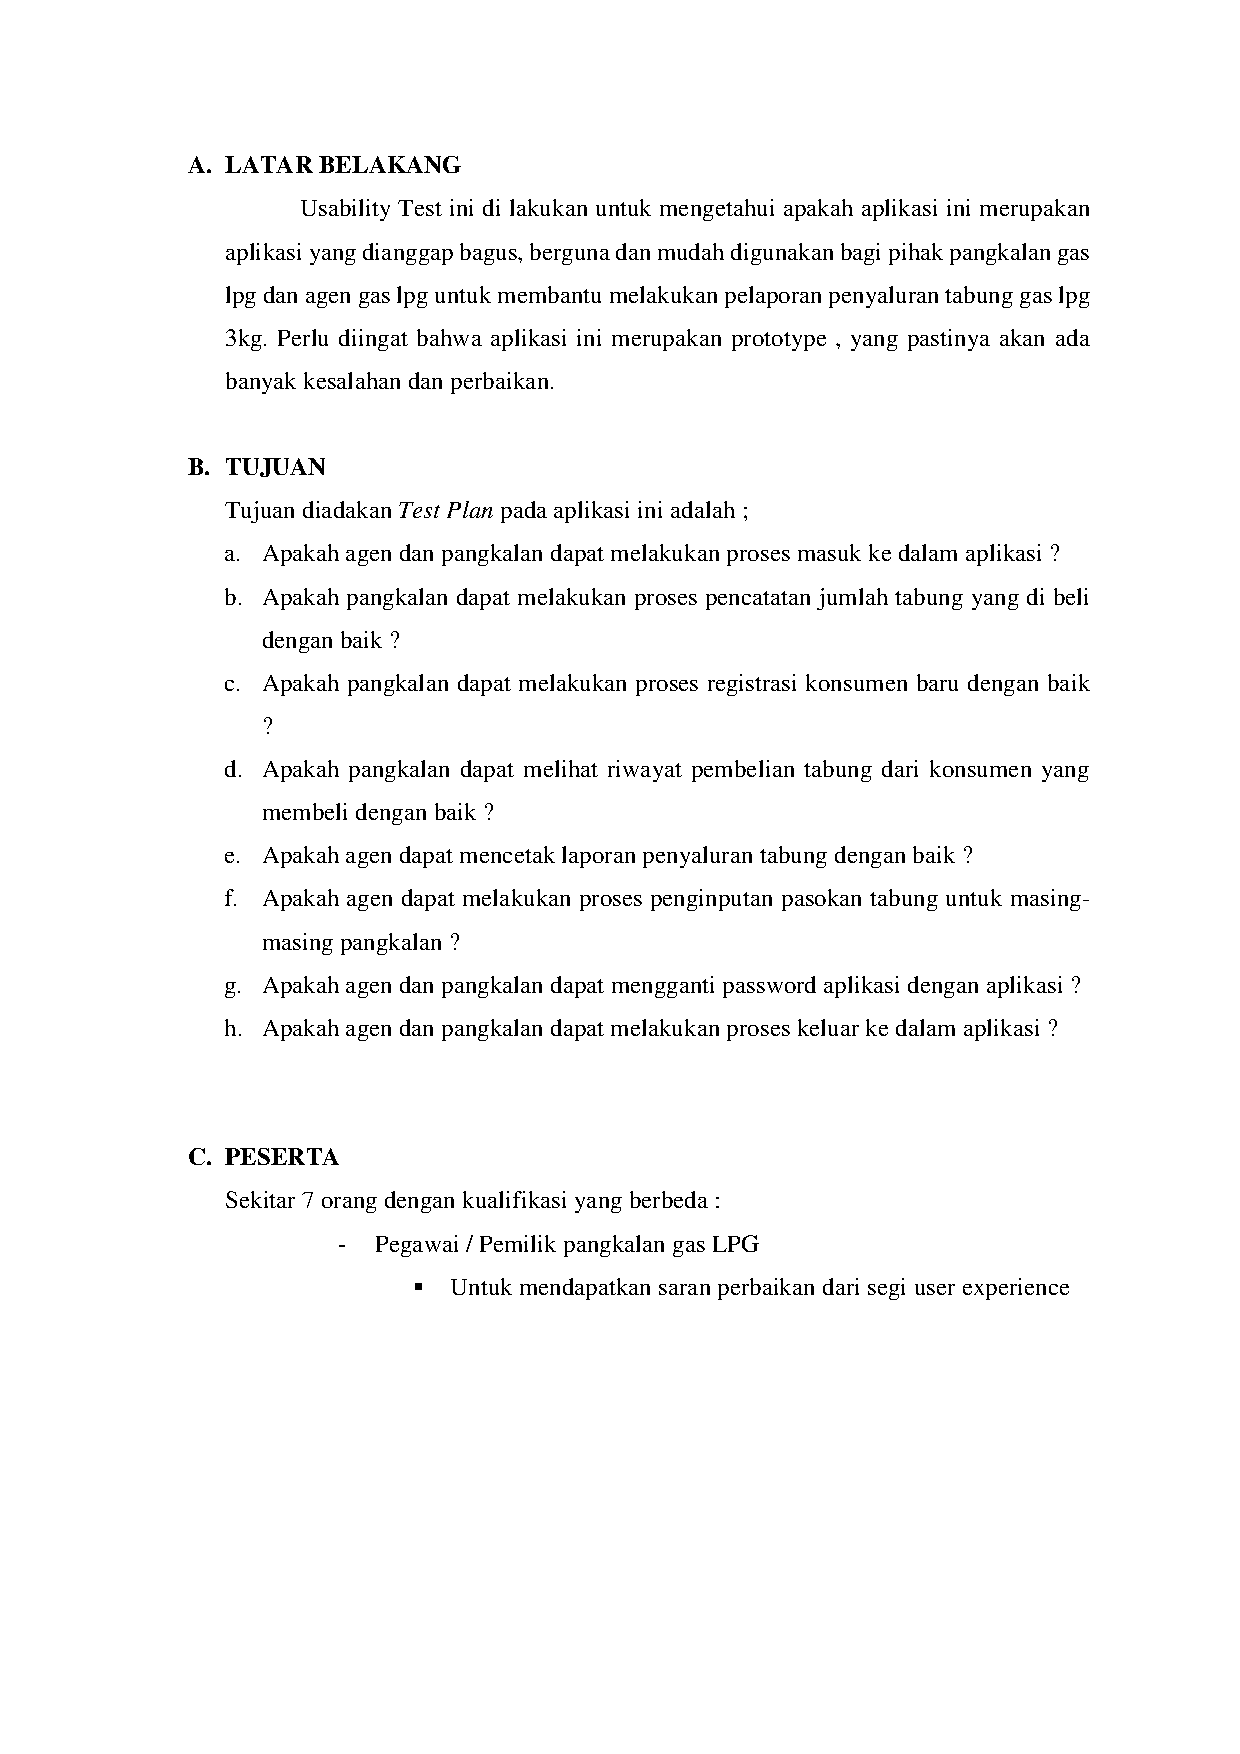
\includepdf[pages=1,scale=.8,pagecommand={
% 	\addcontentsline{toc}{chapter}{LAMPIRAN 4} 
% 	\chapter*{Lampiran 4}
% 	\newappendix{Lampiran 4. Laporan Hasil Pengujian \textit{Usability}}
% },linktodoc=true]{laporan_usability}
% \includepdf[pages=2-,scale=.8,pagecommand={},linktodoc=true]{laporan_usability}
% Lampiran 4 Laporan Usability

% 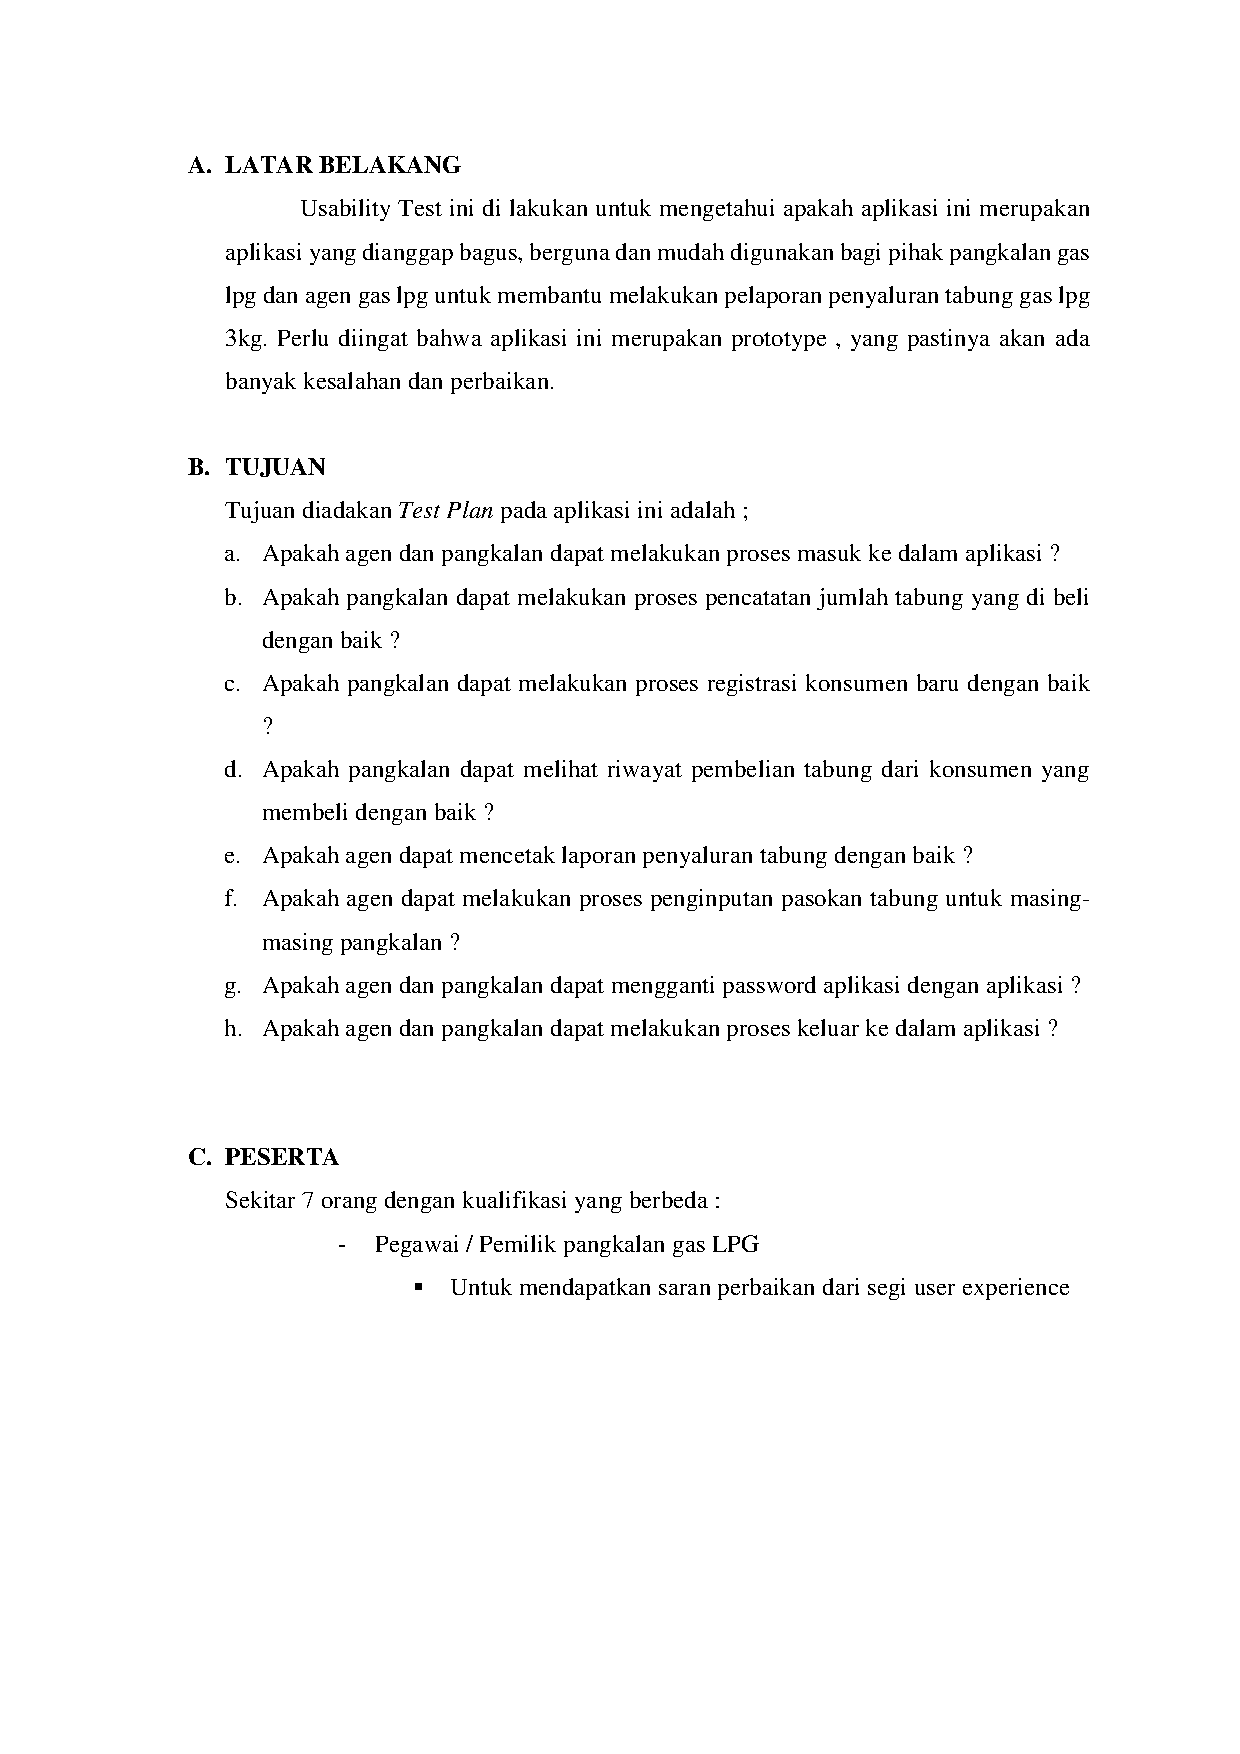
\includepdf[pages=1,scale=.8,pagecommand={
%       \addcontentsline{toc}{chapter}{LAMPIRAN 4}
%       \chapter*{Lampiran 4}
%       \newappendix{Lampiran 4. Laporan Hasil Pengujian \textit{Usability}}
%     },linktodoc=true]{laporan_usability}
% \includepdf[pages=2-,scale=.8,pagecommand={},linktodoc=true]{laporan_usability}